%\documentclass{ctexart}
\documentclass{ctexrep}

\usepackage{amsmath,amsthm,extarrows,color,enumitem,framed,markdown,amscd}
\usepackage[a4paper, left = 2cm, right = 2cm]{geometry}
\usepackage{mathpartir}
\usepackage{unicode-math}
\setmathfont{Latin Modern Math}
%\setmathfont[range=\mathbb]{TeX Gyre Termes Math}
\DeclareMathAlphabet{\mathcal}{OMS}{cmsy}{m}{n}
\let\mathbb\relax % remove the definition by unicode-math
\DeclareMathAlphabet{\mathbb}{U}{msb}{m}{n}
%\setmathfont[range={\mathcal,\mathbfcal},StylisticSet=1]{XITS Math}
%\setmathfont[range=\mathscr]{XITS Math}
\usepackage{newunicodechar}
\newunicodechar{ℝ}{\mathbb{R}}
\newunicodechar{ℚ}{\mathbb{Q}}
\newunicodechar{ℤ}{\mathbb{Z}}
\newunicodechar{ℂ}{\mathbb{C}}

\usepackage{bbm}

\usepackage{tikz-cd}

\usepackage{ulem}

\usepackage{hyperref}
\hypersetup{
     colorlinks   = true,
     linkcolor=blue,
     citecolor=red,
     %filecolor=magenta,      % color of file links
     urlcolor=cyan
}
\usepackage{cleveref}
\usepackage{microtype}

\usepackage{graphicx}
\graphicspath{{./images/}}

\theoremstyle{plain}
\newtheorem{theorem}{Theorem}[section]
\newtheorem{theorem*}{定理}
\newtheorem{proposition*}[theorem*]{命题}
\newtheorem{corollary*}[theorem*]{推论}
\newtheorem{lemma*}[theorem*]{引理}
\newtheorem{definition*}[theorem*]{定义}
\newtheorem{corollary}[theorem]{Corollary}
\newtheorem{lemma}[theorem]{引理}
\newtheorem{proposition}[theorem]{Proposition}

\theoremstyle{definition}
%\newtheorem{definition*}{定义}
\newtheorem{definition}[theorem]{定义}
\newtheorem{example}[theorem]{例}

\theoremstyle{remark}
%\newtheorem*{remark}{注意}
\newtheorem{remark}[theorem]{注意}
\newtheorem*{perspective}{Perspective}

\providecommand{\tightlist}{%
  \setlength{\itemsep}{0pt}\setlength{\parskip}{0pt}}

\newcommand{\bfP}{\mathbf{P}}
\newcommand{\calC}{\mathcal{C}}
\newcommand{\calE}{\mathcal{E}}
\newcommand{\calS}{\mathcal{S}}
\newcommand\calF{\mathcal{F}}
\newcommand{\yoneda}{\mathbf{y}}

\newcommand{\VarTop}{\mathbf{VarTop}}
\newcommand{\Comm}{\mathbf{Comm}}
\newcommand{\id}{\mathrm{id}}
\newcommand{\Aff}{\mathbf{Aff}}
\newcommand{\Diff}{\mathbf{Diff}}
\newcommand{\Open}{\mathbf{Open}}
\newcommand{\op}{\mathrm{op}}
\newcommand{\true}{\mathrm{true}}
\newcommand{\UG}{\mathbf{U}}
\newcommand{\rmH}{H}
\newcommand{\Gposet}{G\text{-}\mathbf{poset}}
\newcommand{\calP}{\mathcal{P}}
\newcommand{\PG}{\calP\rtimes G}
\newcommand{\kPG}{k\PG}
\newcommand{\EI}{\mathrm{EI}}
\newcommand\frakm{\mathfrak{m}}
\newcommand\pgrhp{\pi_{\gamma}r_P^H}
\newcommand\barN{\overline{N}}
\newcommand\Cl{\mathrm{Cl}}
\newcommand\Tr{\mathrm{Tr}}
\newcommand{\abs}[1]{\left\lvert\#1\right\rvert}
\newcommand\calO{\mathcal{O}}
\newcommand\calU{\mathcal{U}}
\newcommand\OGb{\OG b}
\newcommand\ZOG{\mathbf{Z}\OG}
\newcommand\OGG{(\OG)^G}
\newcommand\Irr{\mathrm{Irr}}
\newcommand\Proj{\mathrm{Proj}}
\newcommand\ksng{k_{\sharp}\widehat{\overline{N}}_G}
\newcommand\LP{\mathcal{LP}}
\newcommand\Res{\mathrm{Res}}
\newcommand\ResNCGPVg{\Res_{\overline{C}_G(P)}^{\overline{N}_G(P_{\gamma})}(V(\gamma))}
\newcommand\BOG{\mathbf{B}(\OG)}
\newcommand\pSubGrp{\mathrm{psGrp}}
\newcommand\GL{\mathrm{GL}}
\newcommand\PGL{\mathrm{PGL}}
\newcommand\Inn{\mathrm{Inn}}
\newcommand\std{\mathrm{std}}
\newcommand\bfZ{\mathbf{Z}}
\newcommand\kP{k\calP}
%\newcommand\Mor{\mathrm{Mor}}
\newcommand\Bas{\mathrm{Bas}}
\newcommand\Orb{\mathrm{Orb}}
\newcommand\calB{\mathcal{B}}
\newcommand\Br{\mathrm{Br}}
\newcommand\Image{\mathrm{Im}}
\newcommand\calD{\mathcal{D}}
\newcommand\Ker{\mathrm{Ker}}
\newcommand\bbF{\mathbb{F}}
\newcommand\bbI{\mathbb{I}}
\newcommand\ttI{\mathtt{I}}
\newcommand\Rad{\mathrm{Rad}}
\newcommand\Soc{\mathrm{Soc}}
\newcommand\Perm{\mathrm{Perm}}
\newcommand\bbA{\mathbb{A}}
\newcommand\rmP{\mathrm{P}}
\newcommand\Fam{\mathbf{Fam}}
\newcommand\rmOb{\mathrm{Ob}}

\newcommand\rmMor{\mathrm{Mor}}
\newcommand\rmType{\mathrm{Type}}
\newcommand\rmTerms{\mathrm{Terms}}
\newcommand\Ty{\mathtt{Ty}}
\newcommand\Ter{\mathtt{Ter}}
\newcommand\sfp{\mathsf{p}}
\newcommand\sfq{\mathsf{q}}
\newcommand\bfone{\mathbf{1}}
\newcommand\Psh{\mathrm{Psh}}
\newcommand\Set{\mathbf{Set}}
\newcommand\C{\mathbf{C}}
\newcommand\Sets{\mathbf{Sets}}
\newcommand\Cube{\square^{\op}}
\newcommand\hatcube{\widehat{□}}
\newcommand\hatsquare{\widehat{□}}
\newcommand\cubicalsets{\widehat{□}}
\newcommand\cSets{[\square^{\op},\Sets]}
\newcommand\Setspointed{\mathbf{Sets}_{\kappa}^{\bullet}}
\newcommand{\qq}{\mathtt{q}}
\newcommand{\pp}{\mathtt{p}}
\newcommand{\Cof}{\mathtt{Cof}}
\newcommand{\dec}{\mathrm{dec}}
\newcommand{\fib}{\mathtt{fib}}
\newcommand{\ttzero}{\mathtt{0}}
\newcommand{\ttone}{\mathtt{1}}

\DeclareMathOperator\Obj{Obj}
\DeclareMathOperator\inl{inl}
\DeclareMathOperator\inr{inr}
\DeclareMathOperator\ob{ob}
\DeclareMathOperator\pt{pt}
\DeclareMathOperator\osf{sf}
\DeclareMathOperator\supp{supp}
\DeclareMathOperator\Sub{Sub}
\DeclareMathOperator\Mor{Mor}
\DeclareMathOperator\Colim{Colim}
\DeclareMathOperator\colim{colim}
\DeclareMathOperator\im{im}
\DeclareMathOperator\Pre{Pr}
\DeclareMathOperator\Hom{Hom}
\DeclareMathOperator\Sh{Sh}
\DeclareMathOperator\Spec{Spec}
\DeclareMathOperator\End{End}
\DeclareMathOperator\Aut{Aut}
\DeclareMathOperator\Func{Func}
\DeclareMathOperator\cof{cof}
\DeclareMathOperator\obj{obj}

\newcommand{\DM}{\mathbf{DM}}
\newcommand{\dM}{\mathsf{dM}}
\newcommand{\yc}{\yoneda c}
\newcommand{\yb}{\yoneda b}
\newcommand{\yd}{\yoneda d}
\newcommand{\yone}{\yoneda[1]}
\newcommand{\one}{\mathbf{1}}
\newcommand{\bbmone}{\mathbbm{1}}
\newcommand{\two}{\mathbbm{2}}

\newcommand{\ax}[1]{\mathbf{ax_{#1}}}
\newcommand{\ul}{{\scalebox{0.4}[0.4]{\_}}}
\newcommand{\II}{\mathbb{I}}
\newcommand{\Om}{\Omega}
\newcommand{\cube}{\square}

\newcommand{\forces}{\Vdash} % Kripke-Joyal forcing symbol
\newcommand{\valid}{\vdash} % Internal validity symbol

%\setlength{\parindent}{0pt}

\title{}
\author{}
\date{}

\begin{document}
\chapter{引言}
外延性是这样一个原则：如果两个数学对象具有相同的可观测属性，那么它们就被视为相等。通常，数学的形式系统会包含旨在体现这一原则的公理。在公理集合论的背景下，我们有外延公理，它表明如果两个集合包含相同的元素，那么这两个集合相等。其形式表述为：
\[\forall A . \forall B .((\forall x .(x \in A \Leftrightarrow x \in B)) \Rightarrow A=B)\] 
在（单值/同伦）类型论的语境中，我们有沃沃斯基（Voevodsky）的单值公理[62，第2.10节]，大致来说，该公理表明如果两个类型是同构的，那么它们相等。在类型论的语言中，它可以表述为：
\[\prod_{A, B: U} A \simeq B \to A=B\]
其中\(A \simeq B\)是\(A\)和\(B\)之间等价关系的类型。例如，我们可能有十进制自然数类型\(\mathbb{N}_{dec}\)，其项为\(0, 1, 2, 3, \cdots: \mathbb{N}_{dec}\)，还有二进制自然数类型\(\mathbb{N}_{bin}\)，其项为\(0, 1, 10, 11, \cdots: \mathbb{N}_{bin}\) 。很容易展示如何在这两种编码之间来回转换，也就是说，这两种类型是等价的。因此，根据单值公理，我们可以推断出\(\mathbb{N}_{dec} = \mathbb{N}_{bin}\)。 

乍一看，这些类型相等可能会让人觉得奇怪。例如，7是\(\mathbb{N}_{dec}\)（十进制自然数类型）的一个元素，但不是\(\mathbb{N}_{bin}\)（二进制自然数类型）的元素，那么这两种类型怎么会相等呢？这个公理之所以是自洽的，是因为类型论的规则不允许你构造诸如“7是\(\mathbb{N}_{bin}\)的元素”这样的陈述。这些规则确保所有陈述都以一种适当的通用方式表述，这样一来，陈述就只能利用一个类型的外部可观察到的属性，而不是所使用的特定编码。

我们来看一个类型论中有效陈述的例子：交换幺半群的性质。我们说，类型X构成一个交换幺半群，当且仅当存在一个运算\(\_+\_: X \to X \to X\)，该运算满足结合律、交换律，并且存在一个单位元\(e: X\)。这个定义在类型论中是合理的，因为它适用于任意类型；它对$X$的元素具体是什么样子没有任何假设。 

在类型论中，可以证明\(\mathbb{N}_{dec}\)（十进制自然数类型）构成一个交换幺半群，其中“+”为加法运算，\(e\)为\(0\)。由于\(\mathbb{N}_{dec}\)和\(\mathbb{N}_{bin}\)（二进制自然数类型）只是同一对象（自然数）的不同编码形式，那么\(\mathbb{N}_{bin}\)也应该构成一个交换幺半群。然而，如果没有单值公理，要证明这一点，就需要在两种编码之间来回转换，手动重新构建针对\(\mathbb{N}_{dec}\)的证明过程。单值公理的强大之处在于，由于\(\mathbb{N}_{dec} \simeq \mathbb{N}_{bin}\)，进而\(\mathbb{N}_{dec}=\mathbb{N}_{bin}\)，它能让我们直接将交换幺半群的结构从\(\mathbb{N}_{dec}\)迁移到\(\mathbb{N}_{bin}\) 。 

用这种新的单值性原则扩展类型论的最简单方法，就是将其作为一条公理添加进去。也就是说，假设存在一个项能够证明单值性原则。然而，这种方法存在一个问题。类型论是一个构造性系统，其基本元素具有计算意义。这意味着我们不仅知道如何构造项，还知道如何对这些项进行计算。这种特性的一个例子是，如果我们证明了一个形如 “存在一个自然数$n$使得\ldots” 的命题，那么我们应该能够从这个证明中实际计算出$n$的值。然而，仅仅把单值性作为一条公理提出来，我们无法先验地知道涉及单值性的表达式应该如何计算。 

为了理解这类表达式应如何计算，我们研究单值类型论的模型。一旦我们有了单值类型论（UTT）的模型，我们就有可能通过查看表达式在模型中的解释来计算其值。或者，更有可能的是，我们可以利用该模型来证明新的计算规则的合理性，然后将这些规则添加到类型论中，以恢复良好的计算属性。 

为了理解这类表达式应如何计算，我们研究单值类型论的模型。一旦我们有了单值类型论（UTT）的模型，我们就有可能通过查看表达式在模型中的解释来计算其值。或者，更有可能的是，我们可以利用该模型来证明新的计算规则的合理性，然后将这些规则添加到类型论中，以恢复良好的计算属性。 

单值类型论的首个模型——单纯集模型[39]，本质上利用经典逻辑来判定某些不可判定的命题。因此，虽然它表明单值公理是一致的，但实际上它并不能为恢复类型论的计算内容提供良好基础，因为在该模型中对表达式求值是不可计算的。 

为了解决这些问题，科恩等人引入了类型论的立方体集模型[18]。这个新模型是用构造性元理论构建的，在该模型中对表达式求值是可计算的，从而为恢复类型论的计算内容提供了一种方法。本论文中的大部分工作都基于这个模型展开。 

总的来说，本文使用立方体集拓扑斯的内部语言分析立方体集模型。这种方法具有诸多优势。具体而言，该方法能使立方体集模型的某些方面更加清晰、易于理解；通过对构建单值类型论模型所需的属性进行公理化，我们得以对现有模型进行推广；同时，它还能明确为模拟类型论的各个方面需要哪些属性。

对模型进行公理化的过程并非总是一帆风顺。例如，我们将在第7章中看到，构建单值全域的问题给这种方法带来了特殊挑战。然而，我们认为这样做是一项值得的努力。这种方法为许多应用提供了坚实的基础。例如，在第6章中，我们使用这种方法对单值公理进行了另一种表述。其他作者也将这项工作应用于其他方面，比如证明独立性结果[61]。 

- 在第5章中，我们展示了如何在任何具有适当结构的基本拓扑斯中，使用内部语言对类型论的立方体集模型进行公理化。然而，我们无法定义一个单值全域，尽管我们确实证明了一种与全域无关的单值形式。 

- 在第6章中，我们将单值公理分解为一些替代公理，并表明在具有第5章所规定额外结构的任何拓扑斯中，这些公理都能得到满足。这本质上是对前面提到的与全域无关的单值性证明的一种简化。 

- 在第7章中，我们将解释如何通过一种模态来扩展内部语言，以便能够对拓扑斯的某些全局性质进行公理化。利用这种模态，我们展示如何构建一个单值全域，从而解决前面章节中的不足。 

\chapter{类型论导论}

在本章中，我们将介绍阅读本论文其余部分所需的一些背景知识。特别地，我们将引入单值类型论（也称为同伦类型论），并解释沃沃斯基（Voevodsky）的单值公理。然后，我们将介绍立方体类型论系统，它可被视为标准单值类型论的扩展或细化。立方体类型论的关键特性在于，它为单值公理提供了一种计算解释。 

\section{单值类型论}
单值类型论（UTT），也称为同伦类型论（HoTT），是内涵马丁-洛夫类型论的一个变体。在这个理论中，我们通过引入一个新的公理，即沃沃斯基单值公理，将数学中把同构的结构认为是相等的这样一个常见做法形式化。这样做使我们不得不重新思考内涵类型论中关于等式本质的许多直觉。 

在本节中，我们将回顾马丁-洛夫类型论（Martin-Löf type theory）的基本内容，包括内涵恒等类型的概念，并探讨一种新的直观理解，即把这些恒等类型的元素看作是某个拓扑空间中的路径。我们会发现，这种直观理解使我们对 “任意两个相等性证明本身也相等” 这一原则产生质疑，该原则通常被称为恒等证明的唯一性（UIP）。然后，我们将讨论沃沃斯基（Voevodsky）的单值公理，它体现了这样一种概念：当且仅当两个空间可以相互连续变形时，这两个空间是等价的。最后，我们会看到单值公理实际上与UIP原则是不一致的。 

这里呈现的信息仅作为总结。为避免疑问，我们在此描述的类型论与《同伦类型论》书籍[62]附录A中定义的完全一致。 

\subsection{马丁-洛夫类型论}
马丁-洛夫类型论（MLTT）是一种数学基础体系，它基于类型而非更为常见的集合概念。它允许将命题编码为类型，而这些类型的项则是相关命题的证明。这种解释通常被称为柯里 - 霍华德对应（Curry - Howard correspondence），有时也被称作命题即类型。马丁-洛夫类型论包含许多组件，我们可以用它们来构建和操作类型及项。这些组件包括： 

恒等类型——给定一个类型A以及两个项\(x,y:A\)，我们可以构造出类型\(\mathtt{Id}_{A}(x,y)\)，该类型用于证明\(x\)等于\(y\) 。根据自反性，我们知道任何事物都必然与自身相等，所以对于任意的A以及\(x:A\)，我们都有一个证明\(\mathtt{refl}_{x}:\mathtt{Id}_{A}(x,x)\)，它表明\(x\)等于自身。我们也会将类型\(\mathtt{Id}_{A}(x,y)\)写作\(x =_{A} y\)，或者简写成\(x = y\)。当我们有一个证明\(p:\mathtt{Id}_{A}(x,y)\)时，我们就说\(x\)和\(y\)在命题上相等，这与通过一系列\(\beta\eta\) -归约可相互转换的情况不同，在后一种情况下，我们说它们在定义上相等，并写作\(x \equiv y\)。

\subsection{恒等类型与恒等证明的唯一性（UIP）}
如上文所述，对于任意类型\(A\)以及项\(x,y\in A\)，我们可以构造恒等类型\(\mathtt{Id}_{A}(x,y)\)。我们通过J -消除器来利用恒等证明。这个消除器表明，给定一个依赖于项\(y\in A\)和\(p:x = y\)的类型\(C(x,y,p)\)，我们只需给出一个类型为\(C(x,x,\mathtt{refl}_{x})\)的项，就可以得到\(C(x,y,p)\)的一个实例。或者说，为了证明关于某个与\(x\)命题上相等（由\(p\)见证）的\(y\)的性质\(C\)，只需假设\(y\equiv x\)且\(p\equiv \mathtt{refl}_{x}\) 。 

对类型论的一种标准直觉是，类型代表集合，其项代表该集合的元素。在这种解释下，如果\(x\)和\(y\)不同，我们可能会预期恒等类型对应空集；如果\(x\)和\(y\)实际上代表同一元素，恒等类型则对应单元素集。这让我们可以简单地把自反构造子\(\mathtt{refl}\)解释为单元素集中的唯一元素。理解J-消除器也很容易，因为证明\(p: \mathtt{Id}_{A}(x, y)\)告诉我们\(x\)和\(y\)代表同一元素，并且\(\mathtt{refl}\)和\(p\)都表示单元素集的唯一元素，因此\(C(x, y, p)\)实际上必然与\(C(x, x, \mathtt{refl}_{x})\)表示同一个集合。 

事实上，在这种解释下，由于恒等类型表示的集合最多包含一个元素，那么任何\(p,q:\mathtt{Id}_{A}(x,y)\)实际上必然表示同一个元素。所以我们会期望嵌套恒等类型\(\mathtt{Id}_{\mathtt{Id}_{A}(x,y)}(p,q)\)总是有元素的。这个原则通常被称为恒等证明的唯一性（UIP）。然而，霍夫曼（Hofmann）和施特赖歇尔（Streicher）[29, 32]通过在群胚范畴（每个态射都可逆的范畴）中展示一个模型，表明这个原则并不能从类型论的常规规则推出。在这个模型中：类型被解释为群胚，项\(x,y:A\)被解释为群胚中的元素\(x,y\in \obj A\)，恒等类型\(\mathtt{Id}_{A}(x,y)\)被解释为\(\hom_{A}(x,y)\)上的离散群胚 。UIP原则不成立，因为群胚中两个对象之间可以有多个不同的态射。 

单值类型论（UTT）/同伦类型论（HoTT）的许多工作都受到这样一种直觉的启发：我们不应把类型看作集合、把类型中的项看作集合的元素，而应将类型视为表现得像拓扑空间的对象，其项则是空间中的点。然后，我们把恒等类型的元素\(p: \mathtt{Id}_{A}(x, y)\)视为从点\(x\)到点\(y\)的路径。所以，我们认为\(p\)的行为类似于一个连续函数\(p: \mathbb{I} \to A\)，其中\(\mathbb{I}\)是单位区间\([0, 1]\)，\(p(0) = x\)且\(p(1) = y\)。接着，我们把嵌套恒等类型的元素\(\alpha: \mathtt{Id}_{\mathtt{Id}_{A}(x, y)}(p, q)\)视为同伦\(\alpha: \mathbb{I}×\mathbb{I} \to A\)，使得对于所有\(i \in \mathbb{I}\)，有\(\alpha(0, i) = p(i)\)、\(\alpha(1, i) = q(i)\)，以及\(\alpha(i, 0) = x\)和\(\alpha(i, 1) = y\)。 

在这种类型论的解释下，恒等证明唯一性（UIP）原则似乎不再显而易见。事实上，通过考虑图2.1所示的例子，我们就能明白为什么完全摒弃这一原则是合理的。点\(x\)和\(y\)代表类型\(A\)的两个元素。图中所示的两条路径都是从\(x\)到\(y\)的，因此在这种解释下，它们对应于恒等类型的元素\(p,q:\mathtt{Id}_{A}(x,y)\)。然而，由于空间中心存在空洞，显然在不移动任何一个端点的情况下，无法将其中一条路径连续变形为另一条路径。因此，它们之间不存在同伦，所以，嵌套恒等类型\(\mathtt{Id}_{\mathtt{Id}_{A}(x,y)}(p,q)\)中不存在元素。 
\begin{figure}[htbp]
\centering
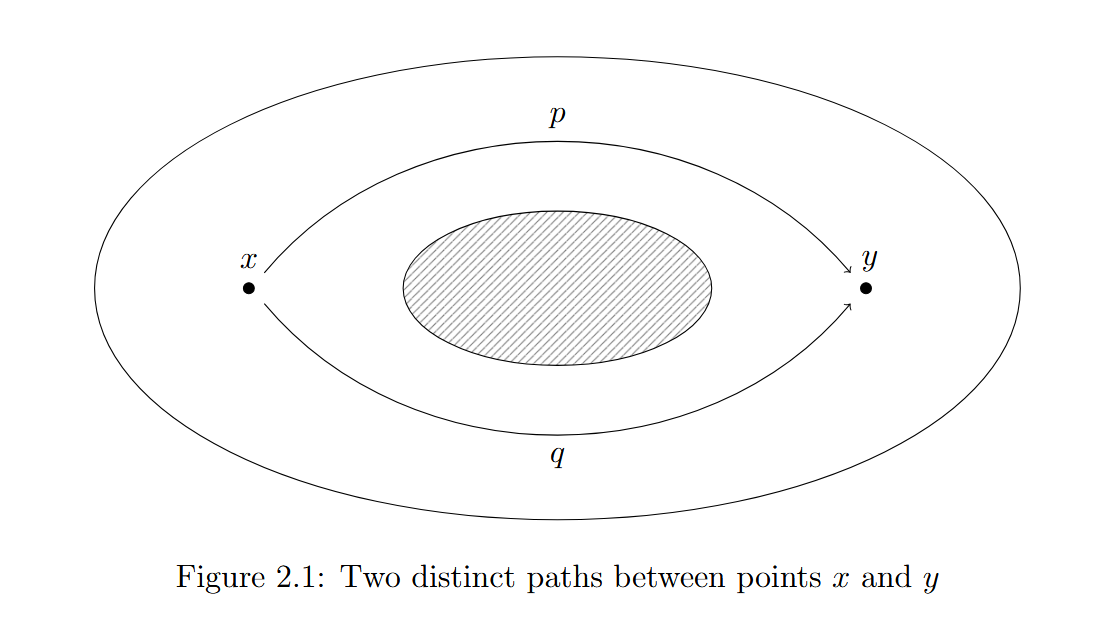
\includegraphics[width=0.75\textwidth]{torus}
\end{figure}

\subsection{沃沃斯基单值公理}
在上一节中，我们讨论了单值类型论（UTT）/同伦类型论（HoTT）背后的新直觉，以及为什么这可能会让我们对恒等证明的唯一性（UIP）原则产生质疑。然而，我们实际上并没有以任何方式扩展类型论，将这种直觉形式化。这是通过沃沃斯基（Voevodsky）的单值公理实现的（见参考文献[62]的2.10节）。该公理将类型之间的相等类型\(\mathtt{Id}_{U}(A, B)\)（也写作\(A = B\)）与等价类型\(A \simeq B\)等同起来。

单值公理体现了一种同伦直观：具有相同同伦群的两个空间（即两个相互等价的空间）在某个分类空间中由一条路径相连。也就是说，我们将\(U\)视为（小）同伦型的分类空间。

从逻辑的角度来看，我们可以把单值公理视为将数学中同构对象视为同一这一常见做法进行形式化的工具。例如，一位数学家可能证明了某个数学对象，比如群\(A\)，与另一个对象\(B\)同构，而我们已经知道\(B\)具有某些性质。接着，这位数学家会在不验证所讨论的性质在同构关系下是否保持的情况下，很自然地得出\(A\)也具有该性质的结论。单值公理通过本质上声明类型论中的每一种构造在等价关系下都保持不变，从而将这种推理形式进行了形式化。 

单值公理的确切表述涉及到一些微妙之处，尤其是关于类型之间等价关系的定义。我们现在给出确切的定义，先从等价关系的定义以及可缩类型这一辅助概念开始。 

定义 2.1.1（可缩性）。如果类型
\[\mathtt{isContr} (A) \triangleq \sum_{a_{0}: A} \prod_{a: A}\left(a_{0}=a\right)\]
有元素，那么称类型\(A\)是可缩的。可缩性表达了这样一个事实，即一个类型有唯一的元素。 

定义 2.1.2（等价关系）。一个等价关系\(A \simeq B\)是一个序对\((f, e)\)，其中\(f: A \to B\)，并且\(e\)是一个证明，它表明对于每一个\(b: B\)，\(f\)在\(b\)处的纤维是可缩的。准确地说：
\[A \simeq B \triangleq \sum_{f: A \to B} \mathtt{isEquiv}(f)\]
其中
\[\fib_{f}(b) \triangleq \sum_{a: A}(f\ a = b)\] 且 \[\mathtt{isEquiv}(f) \triangleq \prod_{b: B} \mathtt{isContr}\left(\fib_{f}(b)\right)\]
对于\(A: U_{i}\)，\(B: U_{j}\)，其中\(i\)、\(j\)为任意值。 

等价关系的一个简单例子是对于任意类型\(A\)的恒等函数\(id_{A}: A \to A\)。为了证明\(id_{A}\)是一个等价关系，我们必须证明\(\prod_{a: A} \mathtt{isContr} (\sum_{x: A}(x = a))\)，利用J-消除器很容易证明这一事实。 

请注意，存在许多相互竞争的等价概念（见参考文献[62]的第4章）。我们选择了这里所使用的这个定义，是因为它简化了第6章中的一些证明。同样值得注意的是，在单值类型论（UTT）中，传统的同构定义并不是一个表现良好的等价概念。具体来说，将\(isEquiv(f)\)定义为存在一个映射\(g: B \to A\)，使得\(\prod_{a: A} g(f a)=a\)且\(\prod_{b: B} f(g b)=b\)，这种定义方式表现欠佳。这是因为这个被称为拟逆的概念并非一个简单的命题（见参考文献[62]的定理4.1.3），因此可能存在多个不同的证明来表明\(f\)具有一个拟逆。这会带来一些不良后果。例如，拟逆等价的类型并非类型\(A \to B\)的子类型，而且事实上，使用拟逆等价来陈述的单值公理是不一致的（见参考文献[62]的练习4.6）。 

接下来，需注意的是，从两个类型之间的相等关系类型到它们之间的等价关系类型，总是存在一个典范映射。 

定义 2.1.3（\textbf{idtoeqv}）。对于所有的\(i\)，以及类型\(A,B: U_{i}\)，存在一个典范映射\(\mathtt{idtoeqv}: (A = B) \to (A \simeq B)\)，它是通过对证明\(A = B\)进行路径归纳法\footnote{这只不过是2.1.2节中所描述的J消除器。我们使用这个名称是考虑到将相等性证明看作路径的这种直观概念。 }来定义的：
\[\mathtt{idtoeqv} \left(\mathtt{refl}_{A}\right) \triangleq id_{A}\]
其中\(id_{A}: A \simeq A\)是被视为等价关系的恒等映射。

最后，我们将单值公理形式化为这样一个陈述：上述映射（\(\mathtt{idtoeqv}\)）本身就是一个等价关系。 

定义 2.1.4（沃沃斯基单值公理）。对于全域\(U_{i}\) 的单值公理断言，对于所有\(A, B \in U_{i}\)，映射\(\mathtt{idtoeqv}: (A = B) \to (A \simeq B)\) 是一个等价关系。 

请注意，单值公理是关于特定全域\(U_{i}\)的一个陈述。一般来说，在单值类型论（UTT）中进行研究时，除非另有明确说明，我们假定所有的全域都是单值的。正是这一假设，将单值类型论/同伦类型论与普通的马丁-洛夫类型论区分开来。 

\subsection{函数外延性}
我们现在回顾一下类型论中的函数外延性原则： 

定义2.1.5（函数外延性）。函数外延性原理表明，对于两个函数\(f, g: \prod_{x: A} B(x)\)，只要它们逐点相等，那么这两个函数就相等。也就是说，我们有这样一个映射：
\[f \approx g \to f = g\qquad\text{其中}\qquad f \approx g \triangleq \prod_{x: A} f(x) = g(x)\]
当我们假定存在这样一个项时，我们就说我们“假定了函数外延性”：
\[\mathtt{funext}_{i, j}: \prod_{A: U_{i}} \prod_{B: A \to U_{j}} \prod_{f, g: \Pi_{x: A} B(x)} f \approx g \to f=g\]
对于所有的全域层级\(i\)和\(j\) 。 

请注意，函数外延性无法从标准的马丁-洛夫类型论的规则中推导得出。然而，它却可以从单值公理中推导出来（见参考文献[62]的4.9节）。 

\subsection{单值公理的另一种表述形式}

虽然定义2.1.4非常简洁，但有时使用单值公理的一种略有不同但等价的表述来进行研究工作会更加容易，我们在此给出这种表述。鉴于以下定义，我们有时会将单值公理称为“真正的单值公理”。 

定义 2.1.6（\textbf{Coerce}）。对于所有的\(i\)，以及类型\(A\)、\(B \in U_{i}\)，我们可以通过路径归纳法，或者按照如下方式来定义一个映射\(\mathtt{coerce} : (A = B) \to A \to B\)：
\[\mathtt{coerce}(p, a) \triangleq \mathtt{fst}(\mathtt{idtoeqv}(p))(a)\]
其中\(\mathtt{fst}\)表示取第一个分量的投影操作。 

定义 2.1.7（朴素单值公理）。对于全域\(U_{i}\) 的朴素单值公理表明，对于所有\(A\)、\(B \in U_{i}\)，存在一个从等价关系到相等关系的映射。换句话说，它断言存在一个属于以下类型的元素：
\[\mathtt{UA}_{i} \triangleq \prod_{A, B: U_{i}} A \simeq B \to A = B\] 

当使用项\(ua : \mathtt{UA}_{i}\)时，我们常常会省略前两个参数（\(A\)和\(B\)）。朴素单值公理的证明可能还会带有一个相关的计算规则。也就是说，存在一个属于类型\(\mathtt{UA}\beta_{i}(ua)\)的元素，其中：
\[\mathtt{UA}\beta_{i}(ua) \triangleq \prod_{A, B: U_{i}} \prod_{f: A \to B} \prod_{e: \mathtt{isEquiv}(f)} \mathtt{coerce}(ua(f, e)) = f\] 

接下来，我们给出一个在单值类型论（UTT）/同伦类型论（HoTT）圈子里广为人知的结果。这一结果将真正的单值公理分解为朴素版本和一条计算规则。需注意，该结果要求函数外延性原理成立。首先，我们给出一个引理，它对这一结果的核心构造进行了推广。 

引理2.1.8。给定\(X: U_{i}\)，\(Y: X \to X \to U_{j}\)以及一个映射\(f: \prod_{x, x': X} x = x' \to Y(x, x')\)，那么对于所有的\(x, x': X\)，\(f\ x\ x'\)是一个等价关系，当且仅当存在一个映射
\[g: \prod_{x, x': X} Y\left(x, x'\right) \to x = x'\]
使得对于所有的\(x, x': X\)以及\(y: Y(x, x')\)，我们有\(f(g(y)) = y\)（我们默认省略\(f\)和\(g\)的前两个参数）。 

定理2.1.9。假设函数外延性成立，那么朴素单值公理连同一条计算规则在逻辑上等价于真正的单值公理。也就是说，存在项
\[ua: \mathtt{UA}_{i}, \qquad ua\beta: \mathtt{UA}\beta_{i}(ua)\]
当且仅当对于所有类型\(A, B \in U_{i}\)，映射\(\mathtt{idtoeqv}: (A = B) \to (A \simeq B)\)是一个等价关系。 

\chapter{马丁-洛夫类型论的模型}

在上一章中，我们讨论了马丁-洛夫类型论以及它的各种扩展，比如单值公理，还有立方体相关的特性，如区间和合成运算。在本章中，我们将描述如何构建马丁-洛夫类型论的范畴模型，并探讨立方体集合范畴中的一个特定模型，该模型将对2.2节中描述的所有扩展进行建模，从而为单值公理提供一个模型。 

\section{范畴族（CwFs）}

对于如何呈现依赖类型理论的模型，存在许多不同的概念。在本论文中，我们将采用迪布耶（Dybjer）提出的范畴族（CwF）概念[23]。我们使用的符号与迪布耶的略有不同，并且将他定义中属于族范畴的函子拆分为两个不同的函子，但除此之外，定义保持不变。我们首先回顾一下预层\(P: \C^{op} \to \Set\)的元素范畴的定义。

定义3.1.1（元素范畴）。给定任意预层\(P: \C^{op} \to \Set\)，\(P\)的元素范畴记为\(\int P\)，其对象为形如\((X, p)\)的对，其中\(X \in \C\)且\(p \in P(X)\)。态射\(f: (X, p) \to (X', p')\)就是\(\C\)中从\(X\)到\(X'\)的态射，并且满足\(P(f)(p') = p\)。 

定义3.1.2（范畴族）。一个范畴族由以下数据构成：
\begin{itemize}
  \item 一个上下文范畴$\C$，其对象代表类型论中的上下文，态射代表上下文之间的替换。这个范畴必须有一个终对象$1$，它代表空上下文。 
  \item 一个函子$\Ty:\C^{op}\to \Set$，它给每个上下文$\Gamma$指定一个集合$\Ty(\Gamma)$，该集合表示上下文$\Gamma$中的类型。对于任意态射$\gamma:\Delta\to\Gamma$以及类型$A\in \Ty(\Gamma)$， $\Ty$ 作用于态射的操作给出了替换的解释，我们用 $A[\gamma]$ 来表示 $\Ty(\gamma)(A) \in \Ty(\Delta)$，这样的表示很直观。$\Ty$ 的函子性质确保了替换是严格可结合的。
  \item 一个函子$\Ter: (\int \Ty)^{op} \to \Set$，它为每个上下文$\Gamma$以及$\Gamma$中的类型$A \in \Ty(\Gamma)$分配一个集合$\Ter(\Gamma, A)$，该集合表示在上下文$\Gamma$中类型为$A$的项。我们将$\Ter(\Gamma, A)$这个集合写作$\Ter(\Gamma \vdash A)$ 。同样，$\Ter$作用于态射的方式严格结合地模拟了替换操作。给定$\gamma: \Delta \to \Gamma$、$A \in \Ty(\Gamma)$以及$a \in \Ter(\Gamma \vdash A)$，我们把$\Ter(\gamma)(a) \in \Ter(\Delta \vdash A[\gamma])$写作$a[\gamma]$。
  \item 一种上下文扩展操作$\_.\_$，它以一个属于$\C$的上下文$\Gamma$和一个属于$\Ty(\Gamma)$的类型$A$为输入，返回一个属于$\C$的对象$\Gamma.A$。同时存在一个态射$\pp: \Gamma.A \to \Gamma$，它代表上下文弱化；还有一个项$\qq \in \Ter(\Gamma . A \vdash A[\pp])$，代表新添加的类型为$A$的变量。这种操作必须满足以下泛性质：对于任何从$\Delta$到$\Gamma$的替换$\gamma$以及属于$\Ter(\Delta \vdash A[\gamma])$的项$a$，都存在唯一的态射$\langle\gamma, a\rangle: \Delta \to \Gamma . A$，使得$\pp \circ\langle\gamma, a\rangle=\gamma$且$\qq[\langle\gamma, a\rangle]=a$。 
\end{itemize}

\section{类型论的预层模型}
在本节中，我们将展示任意预层范畴\(\widehat{\C} = \Set^{\C^{op}}\) 是如何具备范畴族结构的。按照[18]中使用的符号表示法，我们用\(I\)、\(J\)、\(K\)表示范畴\(\C\)的对象，用\(f\)、\(g\)、\(h\)表示范畴\(\C\)的态射。

\section{立方集模型}
在本节中，我们将概述科恩（Cohen）等人[18]提出的类型论的预层模型，该模型对2.2节中讨论的立方类型论的所有特征进行了建模。 

回想一下，德摩根代数是一种分配格，配备了一个函数\(d \mapsto 1 - d\)，该函数是对合的（即\(1 - (1 - d) = d\)），并且满足德摩根定律\(1 - (d_1 \lor d_2) = (1 - d_1) \land (1 - d_2)\)；详见[9，第十一章]。德摩根代数的同态是一种保持有限交、并以及对合函数的函数。令\(\DM\)表示德摩根代数和同态构成的范畴，\(\dM(I)\)表示集合\(I\)上的自由德摩根代数。

定义3.3.1（立方体范畴，\(\square\)）。固定一个可数无限集\(\mathbb{D}\)，其元素我们称为名称，记作\(i\)，\(j\)，\(k\)，… 。\(\square\)的对象是\(\mathbb{D}\)的有限子集，我们记作\(I\)，\(J\)，\(K\)，… 。态射\(\square(I, J)\)是所有从\(J\)到\(\dM(I)\)的函数。这样的函数与从\(\dM(J)\)到\(\dM(I)\)的德摩根代数同态一一对应，并且对于\(f\in\square(I, J)\)和\(g\in\square(J, K)\)，在\(\square\)中的复合是集合范畴中\(g: K \to \dM(J)\)与对应于\(f\)的从\(\dM(J)\)到\(\dM(I)\)的同态的复合 。

因此，\(\square\)等价于德摩根代数范畴（\(\DM\)）的全子范畴的对偶范畴，该全子范畴的对象是有限生成的自由德摩根代数。 因此，作为一种劳威尔理论（Lawvere theory）[41, 2]，它是德摩根代数的代数理论：它是一个具有有限积的范畴，配备了一个内部德摩根代数（对于某个选定的\(i \in \mathbb{D}\)，其基础对象是\(\{i\}\) ），并且在这类范畴中具有泛性质。 

定义3.3.2。一个立方集是立方体范畴上的一个预层。 

立方集范畴\(\Set^{\square^{op}}\)构成了一个范畴族（CwF）的上下文范畴，这将使我们能够解释立方类型论的所有特征。在后续章节中我们将对这个范畴的某些性质进行公理化处理，并以公理化的方式证明前面的陈述。在本节的剩余部分，我们将非常简要地概述科恩等人在文献[18]中所采用的原始方法。

我们首先引入一些在本节中会用到的符号表示。对于任意属于范畴\(\square\)的符号集合\(I\)以及不属于\(I\)的符号\(i\)，我们将\(I,i\)写作\(I \cup \{i\}\)的缩写形式。我们还将\((i0)\)记为从\(I\)到\(I,i\)的映射，该映射将\(i\)映射到\(0\)，而在其他地方是恒等映射。类似地，我们将\((i1)\)记为从\(I\)到\(I,i\)的映射，它将\(i\)映射到\(1\)。这里\(0\)和\(1\)是自由德摩根代数\(\dM(I)\)中的最小元和最大元。最后，我们将\(s_{i}: I,i \to I\)记为包含映射\(I \subseteq \dM(I, i)\) 。 

在接下来的章节中，我们使用\(\Ty\)、\(\Ter\)和\(\_.\_\)来表示立方集范畴上的标准范畴族（CwF），如定义3.2.1中所描述的那样。

\subsection{区间与面格}

\chapter{拓扑斯的内部类型论}

\chapter{在拓扑斯中给出立方类型论模型需要的公理}

在第4章中，我们看到了每个拓扑斯（topos）如何容纳一种基于外延型马丁-洛夫类型论（extensional Martin-Löf type theory）的丰富内部语言。在本论文的其余部分，我们将展示第3.3节中描述的立方类型论模型如何使用这种内部语言来呈现。在此过程中，我们隐式地将Cohen等人[18]给出的模型推广到任何具有适当结构的拓扑斯。为了具体说明这种附加结构，我们采取了一种公理化方法，给出了一组我们要求在内部语言中成立的公理。我们对该模型的表述随后利用了这些公理，而不是假设我们总是在第3.3节描述的拓扑斯中工作。

这种方法有几个优点。首先，它能让我们更好地理解立方集合拓扑斯的哪些性质使其适合用于建模立方类型论；哪些性质是本质的，哪些是多余的。其次，它能让我们确切地看到这些性质是如何被使用的，以及用于哪些构造。例如，我们将看到，某一类命题的封闭性质仅在用于建模$J$-消去子的定义性计算规则时才需要，如果不要求类型论具有这一性质，则可以省去。第三，这种方法使得寻找立方类型论的新模型变得更加容易。这是因为这些公理澄清了拓扑斯为了建模立方类型论必须具备的性质。事实上，在Lawvere理论中存在一个直接且相当明显的模型，由公理的一个子集定义，尽管这实际上与Cohen等人[18]给出的模型非常相似。或者，与其寻找建模立方类型论的新拓扑斯，我们可能想检查现有的感兴趣的拓扑斯，如单纯形集合的拓扑斯[39]，是否也是潜在的模型。利用这里介绍的工作，这项任务被简化为检查拓扑斯的几个简单性质。

\section{公理}

在本节中，我们提出需要在拓扑斯 $\calE$ 的内部类型论中成立的公理。我们对每个公理进行概述，给出其目的的直观解释，并说明它在立方类型论模型构造中的使用位置。这使我们能够看到某些公理仅在用于建模立方类型论的特定部分时才需要，例如定义性相等类型（第5.3.4节）。因此，例如在寻找仅具有命题相等类型的立方类型论模型时，这些公理可以被舍弃。为方便参考，这些公理在本节末尾的图5.4中汇总，使用第4章描述的语言书写。

\subsection{区间$\ttI$}

我们首先公理化建模带有区间对象 $\bbI$ 的类型论所需的结构，如第2.2.1节所述。首先，我们假设存在一个对象 $\ttI:\calU$ ，它将是 $\bbI$ 在模型中的解释。我们假设 $\ttI$ 具有足够的结构来建模区间上的所需运算。具体而言，我们假设 $\ttI$ 配备了态射 $\ttzero,\ttone:1→\ttI$ 和 $\_\sqcap\_, \_\sqcup\_ : \mathtt{I} \to \mathtt{I} \to \mathtt{I}$ ，满足图5.1中的公理 $\ax{1}$--$\ax{4}$。

公理 $\ax{1}$ 表达了区间 $\ttI$ 在内部是连通的，在这个意义上，其元素的任何可判定子集要么是空的，要么是整个 $\ttI$ 。这意味着如果归纳数据类型中的一条路径在路径的某一点具有某种构造子形式，那么它在任何其他点也具有相同的形式。这在第5.3.3节末尾用于证明拓扑斯中的自然数对象是纤维化的（即表示一个类型），以及纤维化在二元余积下封闭。它还在第5.4节中用于证明粘合构造的性质。与公理 $\ax{2}$ 一起，$\ttI$ 的连通性意味着在 $1+1$  中没有从 $\mathtt{inl}\ \ast$ 到 $\mathtt{inr}\ \ast$ 的路径，因此由这些公理确定的马丁-洛夫类型论的路径模型在逻辑上是非退化的。

公理 $\ax{3}$ 和 $\ax{4}$ 赋予 $\ttI$ 一种连接代数（connection algebra）结构[15]。它们捕捉了实数单位区间 $[0,1]$ 上最小值和最大值运算的一些非常简单的性质，这些性质足以确保单例类型的可缩性（第5.2节），并且与后续公理结合，用于定义纤维化从复合的路径提升（见第5.3.1节）。在[18]的模型中，连接代数结构由区间的格结构给出，取 $\_\sqcap\_$ 为二元交（meet），$\_\sqcup\_$ 为二元并（join），并利用 $\ttzero$ 和 $\ttone$ 分别是最小元和最大元这一事实。

\begin{figure}[htbp]
\centering

区间 $\mathtt{I} : \mathcal{U}$ 是连续的
\[
\ax{1} : [\forall (\varphi : \mathtt{I} \to \Omega).\ 
(\forall (i : \mathtt{I}).\ \varphi\,i \lor \neg\varphi\,i) \Rightarrow 
(\forall (i : \mathtt{I}).\ \varphi\,i) \lor (\forall (i : \mathtt{I}).\ 
\neg\varphi\,i)]
\]
有不同的端点 $\ttzero, \ttone : \mathtt{I}$
\[
\ax{2} : [\neg(\ttzero = \ttone)]
\]
有一个连接代数结构
$\_\sqcap\_, \_\sqcup\_ : \mathtt{I} \to \mathtt{I} \to \mathtt{I}$
\[
\ax{3} : [\forall (x : \mathtt{I}).\ \ttzero \sqcap x = \ttzero = x \sqcap \ttzero \land 
\ttone \sqcap x = x = x \sqcap \ttone]
\]
\[
\ax{4} : [\forall (x : \mathtt{I}).\ \ttzero \sqcup x = x = x \sqcup \ttzero \land 
\ttone \sqcup x = \ttone = x \sqcup \ttone].
\]

\caption{区间满足的公理}
\label{fig:interval-axioms}

\end{figure}

\begin{remark}[德摩根对合]
注意，在第 2.2.1 节以及文献 [18] 的模型中，$\mathtt{I}$ 不仅仅是一个格，而且还具有一个对合运算 $1 - (\_) : \mathtt{I} \to \mathtt{I}$（使得 $(1 - (1 - i)) = i$），这使得 
$\sqcup$ 成为 $\sqcap$ 的德摩根对偶，在这个意义上，$i \sqcup j = 1 - ((1 - i) \sqcap (1 - j))$。虽然这种对合结构很方便，但对于接下来的构造来说，它并不是真正必需的。相反，我们只是给出某些概念的 $0$-版本和 $1$-版本；例如，在第 5.3.1 节中的``从 $1$ 复合到 $0$''以及``从 $0$ 复合到 $1$''。
\end{remark}

公理 $\ax{2}$--$\ax{4}$，再加上随后两个公理，将使我们能够证明纤维化提供了 $\Pi$-类型和 $\Sigma$-类型的模型；并且进一步证明由区间对象 $\mathtt{I}$（第 5.2 节）确定的路径类型在命题意义上满足相等类型的规则 [20,63]。

\subsection{上纤维化命题}

接下来，我们需要将立方类型论中面格 $\mathbb{F}$ 的性质公理化。一种方法是假设存在一个具有特定代数性质的对象来建模 $\mathbb{F}$，就像我们在前一节对 $\mathbb{I}$ 所做的那样。然而，我们采取了另一种方法，基于面格的原始直观，即指定一个类 Kan 填充问题的输入，如第 2.2.4 节所述。

Kan 填充以及子空间集合上的其他上纤维化条件，涉及将定义在子空间上的映射扩展到定义在整个空间上的映射。在这里，我们将``空间的子空间''理解为拓扑斯中对象的子对象。由于子对象由到 $\Omega$ 的态射来分类，因此可以考虑由某些命题一般性地指定的子对象集合。更具体地说，给定命题的一个性质 $\mathtt{cof} : \Omega \to \Omega$，我们得到一个相应的命题集合：
\begin{equation}
\Cof \triangleq \{\varphi : \Omega \mid \mathtt{cof}\ \varphi\}
\end{equation}

利用这种直观，我们将面格 $\mathbb{F}$ 内部化为这样一个命题集合。然后我们可以将这个集合的性质公理化，以便构造立方类型论的模型。这些性质展示在图 5.2 中。公理 $\ax{5}$、$\ax{6}$ 和 $\ax{7}$ 与第 2.2.3 节中给出的语法最后四种情况密切对应，该语法生成面格的元素。在这种表述中，$\ax{7}$ 明确表明合取可能是依赖的，这一点在句法表述中并不清晰。公理 $\ax{8}$ 表明上纤维化命题在 $\mathtt{I}$-索引量词下封闭。与 $\ax{7}$ 中的依赖性一样，这不是显式添加到句法表述的面格中的，而是对于定义 $\mathbb{F}$ 的自由生成项集合恰好成立的事实。公理 $\ax{8}$ 用于证明重新对齐引理（引理 5.3.10），该引理用于弱形式粘合的定义中，以确保诱导的纤维化结构扩展到我们正在``粘合''的族上的纤维化结构。

考虑单态射类 $m : A \rightarrowtail B$，其分类态射
\[
\lambda(y : B) \to \exists(x : A).\ m\,x = y : B \to \Omega
\]
通过 $\Cof \rightarrowtail \Omega$ 分解。我们称这样的单态射为上纤维化。类 Kan 填充性质涉及态射 $A \to X$ 何时可以沿着上纤维化 $m : A \rightarrowtail B$ 扩展。相反，在 $\mathcal{E}$ 的内部语言中工作，我们将考虑定义域在 $\Cof$ 中的部分元何时可以扩展到全定义的元。回想一下，在直觉主义逻辑中，类型 $A$ 的部分元通常由子单例表示，即由满足以下条件的函数 $s : A \to \Omega$ 表示：
\[
\forall(x\,x' : A).\ s\,x \land s\,x' \Rightarrow x = x'
\]
然而，使用外延等价的依赖对 $\varphi : \Omega$ 和 $f : [\varphi] \to A$ 将更加方便，如下一定义所示。命题 $\varphi$ 是部分元的范围；用子单例的术语来说，它等于 $\exists(x : A).\ s\,x$。

\begin{definition}[上纤维化部分元，$\square A$]
我们称类型 $\Cof$ 的元素为上纤维化命题。给定类型 $A : \mathcal{U}$，我们定义 $A$ 的上纤维化部分元类型为：
\begin{equation}
\square A \triangleq (\varphi : \Cof) \times ([\varphi] \to A)
\end{equation}

这样一个部分元 $(\varphi, f) : \square A$ 的扩展是一个元素 $a : A$ 连同以下关系的证明：
\begin{equation}
(\varphi, f) \nearrow a \triangleq \forall(u : [\varphi]).\ f\,u = a
\end{equation}
\end{definition}

注意，通过在公理 $\ax{5}$ 中取 $i = 0$，我们有 $\mathtt{cof}(0 = 0)$（即 $\mathtt{cof}\,\top$）和 $\mathtt{cof}(0 = 1)$；将后者与公理 $\ax{2}$ 结合，我们还推导出 $\mathtt{cof}\,\bot$ 成立。因此 $\top$ 和 $\bot$ 都是上纤维化命题，对应于生成面格元素的语法中的前两种情况（第 2.2.3 节）。所以 $A \rightarrowtail A$ 和 $\emptyset \rightarrowtail A$ 总是上纤维化，其中 $\emptyset$ 是始对象。由于 $\mathtt{cof}\,\top$ 成立，对于每个 $a : A$ 存在一个全上纤维化部分元 $(\top, \lambda\_ \to a) : \square A$，其中 $a$ 是扩展 $(\top, \lambda\_ \to a)$ 的唯一元素。由于 $\mathtt{cof}\,\bot$ 成立，每个对象 $A$ 都有一个由 $(\bot, \mathtt{elim}_\emptyset) : \square A$ 给出的空上纤维化部分元，使得每个 $a : A$ 都是 $(\bot, \mathtt{elim}_\emptyset)$ 的扩展。（对于任何 $B : \mathcal{U}$，$\mathtt{elim}_\emptyset : [\bot] \to B$ 表示由 $[\bot]$ 的始性给出的唯一函数。）

\begin{figure}[htbp]
\centering

上纤维化命题 $\Cof = \{\varphi : \Omega \mid \mathtt{cof}\,\varphi\}$（其中 $\mathtt{cof} : \Omega \to \Omega$）

端点等式
\[
\ax{5} : [\forall(i : \mathtt{I}).\ \mathtt{cof}(i = 0) \land \mathtt{cof}(i = 1)]
\]
在二元析取下封闭
\[
\ax{6} : [\forall(\varphi\,\psi : \Omega).\ \mathtt{cof}\,\varphi \Rightarrow \mathtt{cof}\,\psi \Rightarrow \mathtt{cof}(\varphi \lor \psi)]
\]
依赖合取
\[
\ax{7} : [\forall(\varphi\,\psi : \Omega).\ \mathtt{cof}\,\varphi \Rightarrow (\varphi \Rightarrow \mathtt{cof}\,\psi) \Rightarrow \mathtt{cof}(\varphi \land \psi)]
\]
在 $\mathtt{I}$ 上的全称量词
\[
\ax{8} : [\forall(\varphi : \mathtt{I} \to \Omega).\ (\forall(i : \mathtt{I}).\ \mathtt{cof}(\varphi\,i)) \Rightarrow \mathtt{cof}(\forall(i : \mathtt{I}).\ \varphi\,i)]
\]

\caption{上纤维化命题的公理}
\label{fig:cofibrant-axioms}

\end{figure}

\begin{example}
将类型 $\mathtt{I}$ 的变量视为空间中维度的名称是有帮助的，因此在上下文 $i_1, ..., i_n : \mathtt{I}$ 中工作对应于在 $n$ 维中工作。假设我们在具有 $i, j, k : \mathtt{I}$ 的上下文中工作；因此这对应于在三维中工作。我们将元素 $i, j, k : \mathtt{I} \vdash a : A$ 视为空间 $A$ 中的一个立方体，如下所示。令 $\varphi \triangleq (i = 0) \lor (j = 0) \lor (j = 1 \land k = 1)$。由 $\ax{5}$--$\ax{7}$ 我们有 $i, j, k : \mathtt{I} \vdash \varphi : \Cof$。我们将 $\varphi$ 视为指定立方体的某些面和边，在这种情况下是底面 $(i = 0)$、左面 $(j = 0)$ 和前右边 $(j = 1 \land k = 1)$，如下右图所示。那么上纤维化部分元 $f : [\varphi] \to A$ 可以被视为一个部分立方体，仅在 $\varphi$ 指定的区域上有定义。
\begin{figure}[htbp]
\centering
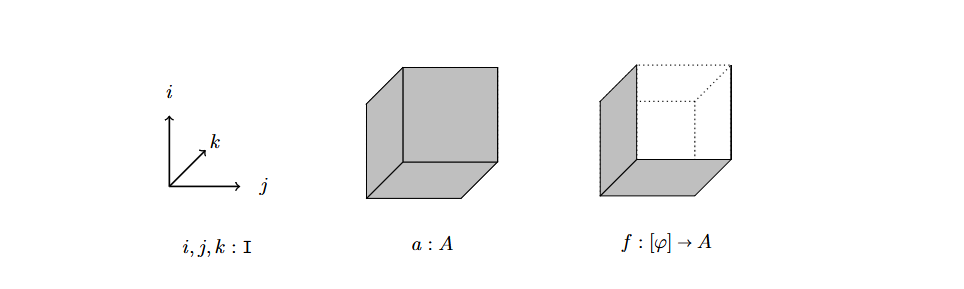
\includegraphics[width=0.9\textwidth]{partial}
%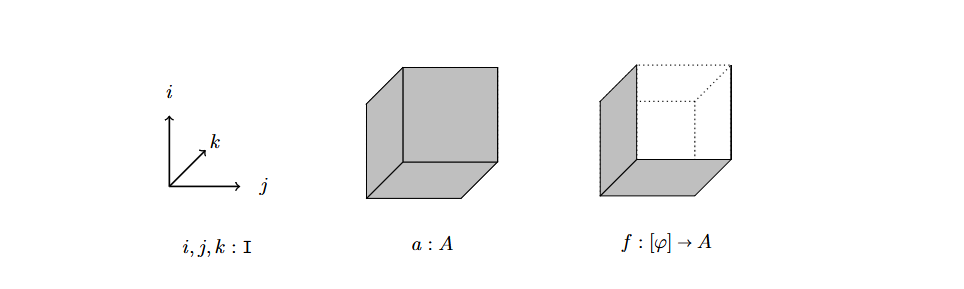
\includegraphics{partial}
\end{figure}
\end{example}

\begin{definition}[相容部分元的并]
称两个部分元 $f : [\varphi] \to A$ 和 $g : [\psi] \to A$ 是相容的，如果它们在都有定义的地方一致：
\begin{equation}
(\varphi, f) \smallsmile (\psi, g) \triangleq \forall(u : [\varphi])(v : [\psi]).\ f\,u = g\,v
\end{equation}

在这种情况下，我们可以形成它们的并 $f \cup g : [\varphi \lor \psi] \to A$，使得：
\[
\forall(u : [\varphi]).\ (f \cup g)\,u = f\,u \qquad \forall(v : [\psi]).\ (f \cup g)\,v = g\,v
\]

为了理解为什么，考虑拓扑斯中的如下推出方：
\[
\begin{tikzcd}
{[\varphi \land \psi]} \arrow[r, tail] \arrow[d,tail] \arrow[dr, phantom, "\_corner" very near end] & {[\psi]} \arrow[d,tail] \arrow[ddr, bend left, "g"] \\
{[\varphi]} \arrow[r, tail] \arrow[drr, bend right, "f"'] & {[\varphi \lor \psi]} \arrow[dr, dashed, "f \cup g" description] \\
& & A
\end{tikzcd}
\]

外方交换是因为 $(\varphi, f) \smallsmile (\psi, g)$ 成立，然后 $f \cup g$ 是从推出诱导的唯一态射。注意，图 5.2 中的公理 $\ax{6}$ 意味着上纤维化部分元的集合在取相容部分元的二元并下封闭。
\end{definition}

以下引理给出了公理 $\ax{7}$ 和 $\ax{8}$ 的另一种刻画。由于我们在上面注意到 $\mathtt{cof}\,\top$ 成立，引理的第 (i) 部分告诉我们上纤维化在综合域论的意义上形成一个优势（dominance）[56]；我们仅在从命题相等类型构造定义性相等类型时使用 $\Cof$ 的这一性质（见第 5.3.4 节）。

\begin{lemma}
\begin{enumerate}
\item[(i)] 公理 $\ax{7}$ 等价于要求上纤维化类在复合下封闭。
\item[(ii)] 公理 $\ax{8}$ 等价于要求上纤维化类在由 $\mathtt{I}$ 的指数化下封闭。
\end{enumerate}
\end{lemma}

\begin{proof}
对于第 (i) 部分，首先假设 $\ax{7}$ 成立，且 $f : A \rightarrowtail B$ 和 $g : B \rightarrowtail C$ 是上纤维化。因此 $\forall(b : B).\ \mathtt{cof}(\exists(a : A).\ f\,a = b)$ 和 $\forall(c : C).\ \mathtt{cof}(\exists(b : B).\ g\,b = c)$ 都成立，我们希望证明 $\forall(c : C).\ \mathtt{cof}(\exists(a : A).\ g(f\,a) = c)$。注意对于 $b : B$ 和 $c : C$：
\begin{align*}
g\,b = c &\Rightarrow (\exists(a : A).\ g(f\,a) = c) = (\exists(a : A).\ f\,a = b) \quad \text{因为 } g \text{ 是单态射} \\
&\Rightarrow \mathtt{cof}(\exists(a : A).\ g(f\,a) = c) = \mathtt{cof}(\exists(a : A).\ f\,a = b) = \top
\end{align*}

因此令 $\varphi \triangleq \exists(b : B).\ g\,b = c$ 和 $\psi \triangleq \exists(a : A).\ g(f\,a) = c$，我们有 $\mathtt{cof}\,\varphi$ 和 $\varphi \Rightarrow \mathtt{cof}\,\psi$。因此由 $\ax{7}$ 我们得到 $\mathtt{cof}(\varphi \land \psi)$，由于 $\psi \Rightarrow \varphi$，这等于 $\mathtt{cof}(\psi)$。所以我们确实有 $\forall(c : C).\ \mathtt{cof}(\exists(a : A).\ g(f\,a) = c)$。

反之，假设上纤维化在复合下封闭，且 $\varphi, \psi : \Omega$ 满足 $\mathtt{cof}\,\varphi$ 和 $\varphi \Rightarrow \mathtt{cof}\,\psi$。$\mathtt{cof}\,\varphi$ 成立等价于单态射 $[\varphi] \rightarrowtail 1$ 是上纤维化；并且由于
\[
\varphi \Rightarrow (\psi = \varphi \land \psi) \Rightarrow (\mathtt{cof}\,\psi = \mathtt{cof}(\varphi \land \psi))
\]
由 $\varphi \Rightarrow \mathtt{cof}\,\psi$ 我们得到 $\varphi \Rightarrow \mathtt{cof}(\varphi \land \psi)$，因此单态射 $[\varphi \land \psi] \rightarrowtail [\varphi]$ 是上纤维化。复合这些单态射，我们有 $[\varphi \land \psi] \rightarrowtail 1$ 是上纤维化，即 $\mathtt{cof}(\varphi \land \psi)$ 成立。

对于第 (ii) 部分，首先假设 $\ax{8}$ 成立，且 $f : A \rightarrowtail B$ 是上纤维化。我们必须证明 $\mathtt{I} \to f : (\mathtt{I} \to A) \rightarrowtail (\mathtt{I} \to B)$ 也是上纤维化。给定 $\beta : \mathtt{I} \to B$ 我们有
\begin{align*}
&(\forall i : \mathtt{I})(\exists a : A).\ f\,a = \beta\,i \\
&\Rightarrow (\forall i : \mathtt{I})(\exists! a : A).\ f\,a = \beta\,i \quad \text{（因为 } f \text{ 是单态射）} \\
&\Rightarrow (\exists \alpha : \mathtt{I} \to A)(\forall i : \mathtt{I}).\ f(\alpha\,i) = \beta\,i \quad \text{（由拓扑斯中的唯一选择）} \\
&\Rightarrow (\forall i : \mathtt{I})(\exists a : A).\ f\,a = \beta\,i
\end{align*}

因此 $(\forall i : \mathtt{I})(\exists a : A).\ f\,a = \beta\,i$ 等于 $(\exists \alpha : \mathtt{I} \to A)(\forall i : \mathtt{I}).\ f(\alpha\,i) = \beta\,i$；并且后者由拓扑斯中的函数外延性等于 $(\exists \alpha : \mathtt{I} \to A).\ (\mathtt{I} \to f)\,\alpha = \beta$。由于 $f$ 是上纤维化，对于每个 $i : \mathtt{I}$ 我们有 $\mathtt{cof}(\exists(a : A).\ f\,a = \beta\,i)$。因此由公理 $\ax{8}$ 我们也有 $\mathtt{cof}((\forall i : \mathtt{I})(\exists a : A).\ f\,a = \beta\,i)$，即 $\mathtt{cof}(\exists \alpha : \mathtt{I} \to A).\ (\mathtt{I} \to f)\,\alpha = \beta)$，正如 $\mathtt{I} \to f$ 为上纤维化所要求的。

反之，假设上纤维化在 $\mathtt{I} \to (\_)$ 下封闭，且 $\varphi : \mathtt{I} \to \Omega$ 满足 $(\forall i : \mathtt{I}).\ \mathtt{cof}(\varphi\,i)$。后者意味着 $\{i : \mathtt{I} \mid \varphi\,i\} \rightarrowtail \mathtt{I}$ 是上纤维化。因此单态射 $(\mathtt{I} \to \{i : \mathtt{I} \mid \varphi\,i\}) \rightarrowtail (\mathtt{I} \to \mathtt{I})$ 也是。由于 $id : \mathtt{I} \to \mathtt{I}$ 在这个单态射的像中当且仅当 $(\forall i : \mathtt{I}).\ \varphi\,i$ 成立，我们有 $\mathtt{cof}((\forall i : \mathtt{I}).\ \varphi\,i)$，正如公理 $\ax{8}$ 所要求的。
\end{proof}

\begin{figure}[htbp]
\centering

严格性公理：任何上纤维化部分类型 $A$

如果在 $A$ 有定义的任何地方都与全类型 $B$ 同构

则可以扩展为一个与 $B$ 同构的全类型 $B'$：
\begin{align*}
\ax{9} : &\{\varphi : \Cof\}(A : [\varphi] \to \mathcal{U})(B : \mathcal{U})(s : (u : [\varphi]) \to (A\,u \cong B)) \to \\
&(B' : \mathcal{U}) \times \{s' : B' \cong B \mid \forall(u : [\varphi]).\ A\,u = B' \land s\,u = s'\}
\end{align*}

\caption{严格性公理}
\label{fig:strictness-axiom}

\end{figure}

\subsection{严格性公理}

我们的最后一个公理与其他公理不同，它与其说是关于公理化立方类型论的某些本质方面，不如说是关于解决内部语言方法的一个弱点。这最后一个公理 $\ax{9}$ 指出，任何上纤维化部分类型 $A$，如果在 $A$ 有定义的任何地方都与全类型 $B$ 同构，则可以扩展为一个与 $B$ 同构的全类型 $B'$。该公理的精确定义在图 5.3 中给出，同构的定义如下：

\begin{definition}[同构]
给定对象 $A, B : \mathcal{U}$，$A$ 和 $B$ 之间的同构是一个具有双边逆的函数 $f : A \to B$。令 $A \cong B$ 为 $A$ 和 $B$ 之间同构的类型，定义为：
\[
A \cong B \triangleq \{f : A \to B \mid (\exists g : B \to A)\, (g \circ f = id) \land (f \circ g = id)\}
\]

我们说 $A$ 和 $B$ 同构，如果存在同构 $f : A \cong B$。我们说两个族 $A, B : \Gamma \to \mathcal{U}$ 同构，如果它们的每个纤维都同构，并且我们滥用记号写作：
\[
A \cong B \triangleq (x : \Gamma) \to A\,x \cong B\,x
\]
\end{definition}

同构在内部类型论的外延相等意义下具有逆，这与我们后面引入的等价概念形成对比，后者仅在路径相等意义下具有逆。此外，这些逆是唯一的，因此，使用唯一选择，我们总能构造同构的逆。因此，给定 $f : A \cong B$，我们将 $f^{-1} : B \cong A$ 写作 $f$ 的这个逆。

为了对这个公理的作用获得一些直观理解，考虑以下例子。我们有一个在区间上的类型族 $B : \mathtt{I} \to \mathcal{U}$ 和一个单一类型 $A : \mathcal{U}$ 使得 $A \cong B\,0$。我们希望能够在某种意义上``覆盖'' $B$ 在 $0$ 处的值，用 $A$ 替换它。这应该给我们一个族 $B' : \mathtt{I} \to \mathcal{U}$，它与原始族 $B$ 同构，但满足 $A = B'\,0$。给定公理 $\ax{9}$，我们可以将 $B'\,i : \mathcal{U}$ 定义为 $\ax{9}\,\{i=0\}\,(\lambda\_ \to A)\,(B\,i)\,(\lambda\_ \to s)$ 的第一个投影，其中 $s : A \cong B\,0$ 是见证 $A$ 在 $0$ 处与 $B$ 同构的同构。第二个投影给出新的同构，见证 $B'$ 与 $B$ 同构，特别是当 $i = 0$ 时这个新的同构就是原来的那个。

先验地，没有公理 $\ax{9}$，在内部类型论中没有办法执行这样的构造。事实上，从范畴论的角度来看，这样的构造似乎相当奇怪，因为我们通常只在``同构意义下''工作。然而，这个公理后面将需要用于验证类型论中必须成立的某些定义性相等。在这个意义上，对公理 $\ax{9}$ 的需求让人想起在范畴模型中将类型论中的替换解释为拉回时出现的一些问题。

公理 $\ax{9}$ 将用于恢复 Cohen 等人 [18] 使用的严格形式的粘合。它在预层模型中的有效性依赖于外部元理论中的一个构造，该构造无法在内部复制；详见定理 5.6.3。

\section{路径类型}

给定 $A : \mathcal{U}$，我们称类型 $\mathtt{I} \to A$ 的元素为 $A$ 中的路径。与 $A$ 关联的路径类型是 $\_\sim\_ : A \to A \to \mathcal{U}$，其中
\begin{equation}
a_0 \sim a_1 \triangleq \{p : \mathtt{I} \to A \mid p\,0 = a_0 \land p\,1 = a_1\}
\end{equation}

这些类型能否用于建模马丁-洛夫相等类型的规则？我们当然可以解释相等引入规则（自反性），因为由常数函数给出的退化路径
\begin{equation}
\mathtt{k}\,a\,i \triangleq a
\end{equation}
满足 $\mathtt{k} : \{A : \mathcal{U}\}(a : A) \to a \sim a$。然而，我们需要进一步的假设来解释相等消去规则，也称为路径归纳，在第 2.1.2 节中描述。Coquand 给出了相等消去的另一种（命题等价的）表述，用替换函数 $a_0 \sim a_1 \to P\,a_0 \to P\,a_1$ 和单例类型 $(a_1 : A) \times (a_0 \sim a_1)$ 的可缩性来表述；见 [11,图2]。连接代数结构给出后者，因为使用 $\ax{3}$ 和 $\ax{4}$ 我们有
\begin{align}
&\mathtt{ctr} : \{A : \mathcal{U}\}\{a_0\,a_1 : A\}(p : a_0 \sim a_1) \to (a_0, \mathtt{k}\,a_0) \sim (a_1, p) \\
&\mathtt{ctr}\ p\ i \triangleq (p\ i, \lambda j \to p(i \sqcap j))\notag
\end{align}

然而，为了得到适当行为的替换函数，我们必须考虑赋予某些额外结构的类型族；并且该结构必须通过类型形成运算（积、函数、相等类型等）提升。这就是下一节定义所实现的内容。

\begin{figure}[htbp]
\centering

区间 $\mathtt{I} : \mathcal{U}$ 是连通的
\[
\ax{1} : [\forall(\varphi : \mathtt{I} \to \Omega).\ (\forall(i : \mathtt{I}).\ \varphi\,i \lor \neg\varphi\,i) \Rightarrow (\forall(i : \mathtt{I}).\ \varphi\,i) \lor (\forall(i : \mathtt{I}).\ \neg\varphi\,i)]
\]

具有不同的端点 $0, 1 : \mathtt{I}$
\[
\ax{2} : [\neg(0 = 1)]
\]

以及连接代数结构 $\_\sqcap\_, \_\sqcup\_ : \mathtt{I} \to \mathtt{I} \to \mathtt{I}$
\[
\ax{3} : [\forall(x : \mathtt{I}).\ 0 \sqcap x = 0 = x \sqcap 0 \land 1 \sqcap x = x = x \sqcap 1]
\]
\[
\ax{4} : [\forall(x : \mathtt{I}).\ 0 \sqcup x = x = x \sqcup 0 \land 1 \sqcup x = 1 = x \sqcup 1]
\]

\vspace{1em}

上纤维化命题 $\Cof = \{\varphi : \Omega \mid \mathtt{cof}\,\varphi\}$（其中 $\mathtt{cof} : \Omega \to \Omega$）

包含端点等式
\[
\ax{5} : [\forall(i : \mathtt{I}).\ \mathtt{cof}(i = 0) \land \mathtt{cof}(i = 1)]
\]

在二元析取下封闭
\[
\ax{6} : [\forall(\varphi\,\psi : \Omega).\ \mathtt{cof}\,\varphi \Rightarrow \mathtt{cof}\,\psi \Rightarrow \mathtt{cof}(\varphi \lor \psi)]
\]

依赖合取
\[
\ax{7} : [\forall(\varphi\,\psi : \Omega).\ \mathtt{cof}\,\varphi \Rightarrow (\varphi \Rightarrow \mathtt{cof}\,\psi) \Rightarrow \mathtt{cof}(\varphi \land \psi)]
\]

在 $\mathtt{I}$ 上的全称量词
\[
\ax{8} : [\forall(\varphi : \mathtt{I} \to \Omega).\ (\forall(i : \mathtt{I}).\ \mathtt{cof}(\varphi\,i)) \Rightarrow \mathtt{cof}(\forall(i : \mathtt{I}).\ \varphi\,i)]
\]

\vspace{1em}

严格性公理：任何上纤维化部分类型 $A$

如果在 $A$ 有定义的任何地方都与全类型 $B$ 同构

则可以扩展为一个与 $B$ 同构的全类型 $B'$：
\begin{align*}
\ax{9} : &\{\varphi : \Cof\}(A : [\varphi] \to \mathcal{U})(B : \mathcal{U})(s : (u : [\varphi]) \to (A\,u \cong B)) \to \\
&(B' : \mathcal{U}) \times \{s' : B' \cong B \mid \forall(u : [\varphi]).\ A\,u = B' \land s\,u = s'\}
\end{align*}

\caption{所有公理}
\label{fig:all-axioms}

\end{figure}

\section{Cohen-Coquand-Huber-Mörttberg（CCHM）纤维化}

在本节中，我们将展示如何把第 3.3.4 节中针对特定预层模型引入的纤维化概念推广到任何具有区间对象的拓扑斯，如前几节所述。为此，我们使用图 5.4 中的\textbf{上纤维化命题}概念来内部化文献 [18] 中描述的复合和填充运算。我们证明这个概念在形成 $\Sigma$-、$\Pi$- 和路径类型以及基本数据类型下封闭；最后我们展示如何定义具有定义性计算规则的等同类型，即 $\mathtt{Id}$-类型，并证明纤维化在形成 $\mathtt{Id}$-类型下也封闭。

\subsection{复合与填充结构}

给定区间索引的类型族 $A : \mathtt{I} \to \mathcal{U}$，我们将依赖函数类型 $\Pi_\mathtt{I} A \triangleq (i : \mathtt{I}) \to A\,i$ 的元素视为\textbf{依赖类型路径}。我们称类型 $\square(\Pi_\mathtt{I} A)$ 的元素为\textbf{上纤维化部分路径}。给定 $(\varphi, f) : \square(\Pi_\mathtt{I} A)$，我们可以在区间的点 $i : \mathtt{I}$ 处求值，得到一个上纤维化部分元 $(\varphi, f) \ @\  i : \square(A\,i)$：
\begin{equation}
(\varphi, f) \ @\  i \triangleq (\varphi, \lambda(u : [\varphi]) \to f\,u\,i)
\end{equation}

在 $A : \mathtt{I} \to \mathcal{U}$ 中\textbf{从 $\ttzero$ 填充}的运算接受任何 $(\varphi, f) : \square(\Pi_\mathtt{I} A)$ 和任何 $a_0 : A\,\ttzero$ 使得 $(\varphi, f) \ @\  \ttzero \nearrow a_0$，并将 $(\varphi, f)$ 扩展为依赖类型路径 $g : \Pi_\mathtt{I} A$ 且满足 $g\,\ttzero = a_0$。这是一种\textbf{均匀同伦扩展与提升性质（HELP）}[49, 第 10 章, 第 3 节] 的形式，用\textbf{上纤维化命题}内部陈述，而非用\textbf{上纤维化}外部陈述。与 Cohen 等人相比，我们内部方法的一个特点是，他们对复合/填充运算的\textbf{均匀性}条件（定义 3.3.4）---这使得可以避免经典 Kan 填充概念 [10] 的非构造性方面---当运算用上纤维化命题的内部集合 $\Cof$ 表述时自动成立。

由于我们不假设区间具有反转路径的任何结构（见备注 5.1.1），我们还需要考虑从 $\ttone$ 填充的对称概念。令
\begin{equation}
\{\ttzero, \ttone\} \triangleq \{i : \mathtt{I} \mid i = \ttzero \lor i = \ttone\}
\end{equation}
注意，由于公理 $\ax{2}$，这与布尔值对象 $1 + 1$ 同构，因此存在一个函数
\begin{equation}
\overline{\phantom{x}} : \{\ttzero, \ttone\} \to \{\ttzero, \ttone\}
\end{equation}
满足 $\overline{\ttzero} = \ttone$ 和 $\overline{\ttone} = \ttzero$。在下文中，我们不使用路径反转，而是用 $e : \{\ttzero, 1\}$ 参数化定义，并使用 (5.10) 来交换 $\ttzero$ 和 $\ttone$。

\begin{definition}[填充结构]
给定 $e : \{0, 1\}$，类型 $\mathtt{Fill}\,e\,A : \mathcal{U}$ 表示 $\mathtt{I}$-索引类型族 $A : \mathtt{I} \to \mathcal{U}$ 的\textbf{填充结构}，定义为：
\begin{align}
\mathtt{Fill}\,e\,A \triangleq &(\varphi : \Cof)(f : [\varphi] \to \Pi_\mathtt{I} A)(a : \{a' : A\,e \mid (\varphi, f) \ @\  e \nearrow a'\}) \to \\
&\{g : \Pi_\mathtt{I} A \mid (\varphi, f) \nearrow g \land g\,e = a\}\notag
\end{align}
\end{definition}

\begin{example}
为了直观理解为什么这样的运算被称为填充，考虑以下例子。为简单起见，假设 $A : \mathtt{I} \to \mathcal{U}$ 是一个常值族 $A \triangleq \lambda(\_ : \mathtt{I}) \to A'$。回想一下，我们将类型 $\mathtt{I}$ 的变量视为空间中的维度；因此，在给定环境上下文 $j, k : \mathtt{I}$ 中的元素 $a : A$，我们将 $a$ 视为空间 $A$ 中的一个正方形。我们希望将这个二维正方形扩展为三维立方体，如下所示。

\begin{figure}[htbp]
\centering
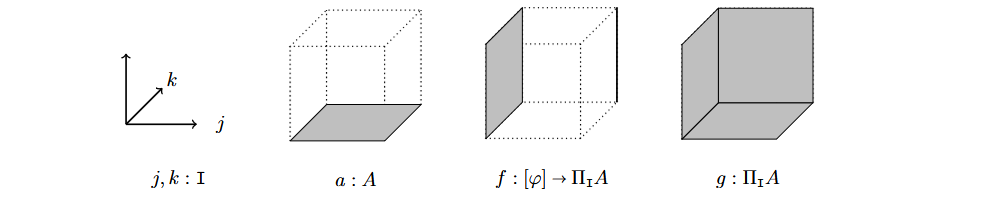
\includegraphics[width=0.9\textwidth]{comp}
\end{figure}

然而，让我们想象我们已经知道如何在立方体的某些面和边上扩展 $a$，例如，在由 $\varphi \triangleq (j = 0) \lor (j = 1 \land k = 1)$ 指定的面/边上。这意味着我们有一个上纤维化\textbf{部分路径} $f : [\varphi] \to \Pi_\mathtt{I} A$，它在两者都有定义的地方与 $a$ 一致，即 $(\varphi, f) \ @\  0 \nearrow a$。注意，$f$ 是一个\textbf{部分路径}而非\textbf{部分元素}，因为在它有定义的面/边上，它必须在所有点上都有定义，沿着我们扩展 $a$ 的新维度，即 $\varphi$ 不能依赖于这个新维度。这个数据的填充是一个立方体 $g : \Pi_\mathtt{I} A$，它与我们从之出发的面/边一致。也就是说，它扩展 $f$ 并在立方体的底部与 $a$ 一致：$(\varphi, f) \nearrow g$ 且 $g\,0 = a$。
\end{example}

与先前工作 [11] 相比，[18] 的一个显著特点是，这样的填充结构可以从更简单的\textbf{复合}结构构造出来，后者仅从上纤维化部分路径一端的扩展产生另一端的扩展。我们将使用公理 $\ax{3}$--$\ax{6}$ 从以下概念推导出这一点，这是本章的主要概念。

\begin{definition}[CCHM 纤维化]
类型 $\Gamma : \mathcal{U}$ 上的 \textbf{CCHM 纤维化} $(A, \alpha)$ 是一个配备纤维化结构 $\alpha : \mathtt{isFib}\,A$ 的族 $A : \Gamma \to \mathcal{U}$，其中 $\mathtt{isFib} : \{\Gamma : \mathcal{U}\}(A : \Gamma \to \mathcal{U}) \to \mathcal{U}$ 定义为：
\begin{equation}
\mathtt{isFib}\,\{\Gamma\}\,A \triangleq (e : \{0, 1\})(p : \mathtt{I} \to \Gamma) \to \mathtt{Comp}\,e\,(A \circ p)
\end{equation}

这里 $\mathtt{Comp} : (e : \{0, 1\})(A : \mathtt{I} \to \mathcal{U}) \to \mathcal{U}$ 是 $\mathtt{I}$-索引族的\textbf{复合结构}类型：
\begin{align}
\mathtt{Comp}\,e\,A \triangleq &(\varphi : \Cof)(f : [\varphi] \to \Pi_\mathtt{I} A) \to \\
&\{a_0 : A\,e \mid (\varphi, f) \ @\  e \nearrow a_0\} \to \{a_1 : A\,\overline{e} \mid (\varphi, f) \ @\  \overline{e} \nearrow a_1\}\notag
\end{align}
\end{definition}

\begin{example}
在例 5.3.2 中，我们考虑了族 $A$ 为常值的情况。我们现在考虑非常值情况，为 CCHM 纤维化定义 (5.12) 中 $\Gamma$ 和 $p : \mathtt{I} \to \Gamma$ 的作用提供一些直观理解。遵循纤维化应该对应于由另一个拓扑空间参数化的拓扑空间这一直观，我们将 $\Gamma$ 视为一个空间，称为\textbf{纤维化的底空间}，将 $p : \mathtt{I} \to \Gamma$ 视为这个空间中的一条\textbf{路径}。对于每个 $x : \Gamma$，我们有一个位于 $x$ 之上的空间 $A\,x$，称为在 $x$ 处的\textbf{纤维}。特别地，我们有位于路径 $p$ 的起点和终点之上的空间 $A(p\,0)$ 和 $A(p\,1)$，如下所示：

% [图示：底空间中的路径 p 和上方的纤维 A(p0)、A(p1)]
\begin{figure}[htbp]
\centering
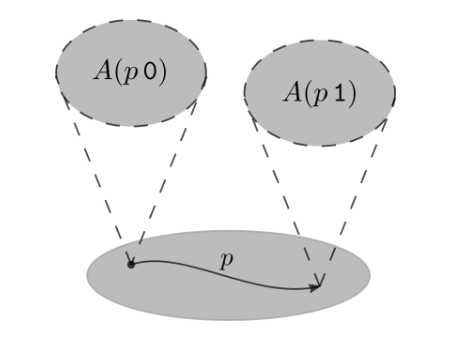
\includegraphics[width=0.3\textwidth]{cchm_fib}
\end{figure}

如例 5.3.2 中一样，考虑在具有两个维度 $j, k : \mathtt{I}$ 的上下文中工作，其中 $\varphi \triangleq (j = 0) \lor (j = 1 \land k = 1)$。进一步，取 $e = 0$。这意味着 $f : [\varphi] \to \Pi_\mathtt{I}(A \circ p)$ 定义了立方体的一个面和一个边，如例 5.3.2 中一样，只是这些不再存在于单个纤维内部，而是存在于 $A$ 的全空间中，位于路径 $p$ 之上，如下左图所示。然后 $a_0$ 在空间 $A(p\,0)$ 中定义了一个正方形，如下中图所示，其中条件 $(\varphi, f) \ @\  e \nearrow a_0$ 确保 $f$ 与 $a_0$ 的相关边和角正确对齐。复合运算的结果，$\alpha\,0\,p\,\varphi\,f\,a_0 : A(p\,1)$，因此在纤维 $A(p\,1)$ 中定义了一个正方形，其中条件 $(\varphi, f) \ @\  \overline{e} \nearrow a_1$ 确保这个正方形与 $f$ 正确对齐，如下右图所示。

% [图示：左图 f : [φ] → Π_I(A ∘ p)，中图 a_0 : A(p0)，右图 α 0 p φ f a_0 : A(p1)]
\begin{figure}[htbp]
\centering
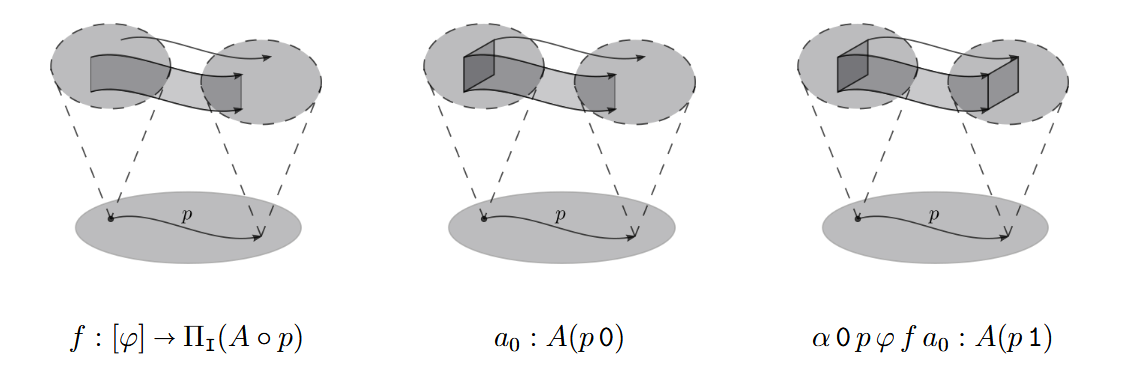
\includegraphics[width=0.9\textwidth]{cchm_fib2}
\end{figure}
\end{example}

\begin{definition}[CCHM 纤维化的 CwF]
令 $\mathtt{Fib}\,\Gamma$ 为对象 $\Gamma$ 上 CCHM 纤维化的类型，定义为：
\begin{equation}
\mathtt{Fib}\,\Gamma \triangleq (A : \Gamma \to \mathcal{U}) \times \mathtt{isFib}\,A
\end{equation}

CCHM 纤维化在重索引下封闭：给定 $\gamma : \Delta \to \Gamma$ 和 $A : \Gamma \to \mathcal{U}$，我们得到一个函数 $\_[\gamma] : \mathtt{isFib}\,A \to \mathtt{isFib}(A \circ \gamma)$，定义为 $\alpha[\gamma]\,e\,p \triangleq \alpha\,e\,(\gamma \circ p)$。因此我们得到一个函数 $\_[\_] : \mathtt{Fib}\,\Gamma \to (\Delta \to \Gamma) \to \mathtt{Fib}\,\Delta$，定义为：
\begin{equation}
(A, \alpha)[\gamma] \triangleq (A \circ \gamma, \alpha[\gamma])
\end{equation}

这是函子性的：$(A, \alpha)[id] = (A, \alpha)$ 且 $(A, \alpha)[g \circ f] = (A, \alpha)[g][f]$。由此可得，$\mathtt{Fib}$ 具有\textbf{带族的范畴（Category with Families）}的结构，通过将族取为每个 $\Gamma : \mathcal{U}$ 上的 CCHM 纤维化 $(A, \alpha) : \mathtt{Fib}\,\Gamma$，并将这种族的元素取为 $(x : \Gamma) \to A\,x$ 中的依赖函数。
\end{definition}

\begin{remark}[纤维化对象]
我们说 $A : \mathcal{U}$ 是一个\textbf{纤维化对象}，如果我们在终对象 $1$ 上的常值族 $\lambda(\_ : 1) \to A$ 有一个纤维化结构。注意，如果 $(A, \alpha) : \mathtt{Fib}\ \Gamma$ 是一个纤维化，那么对于每个 $x : \Gamma$，类型 $A\ x : \mathcal{U}$ 是纤维化的，其纤维化结构由通过映射 $\lambda(\_ : 1) \to x : 1 \to \Gamma$ 重索引 $\alpha$ 给出。然而，其逆不成立：拥有一族纤维化结构，即 $(x : \Gamma) \to \mathtt{isFib}(\lambda(\_ : 1) \to A\ x)$ 的元素，比拥有 $A : \Gamma \to \mathcal{U}$ 的纤维化结构要弱。为了理解为什么，考虑由以下定义的族 $P : \mathtt{I} \to \mathcal{U}$：
\begin{equation}
P\ i \triangleq [0 = i]
\end{equation}

对于每个 $i : \mathtt{I}$，纤维 $P\ i : \mathcal{U}$ 是一个纤维化对象，具有纤维化结构 $\rho_i : \mathtt{isFib}(\lambda(\_ : 1) \to P\ i)$，由 $\rho_i\ e\ p\ \varphi\ f\ x \triangleq x$ 给出。然而，不可能构造 $\rho : \mathtt{isFib}\ P$。因为如果可能，我们可以定义 $\rho\ 0\ id\ \bot\ \mathtt{elim}_\emptyset\ \ast : [0 = 1]$；结合 $\ax{2}$，这将导致矛盾。这个例子将在后面第 7.1 节中更详细地探讨。
\end{remark}

如果 $\alpha : \mathtt{Fill}\ e\ A$，那么 $\lambda\varphi\ f\ a \to \alpha\ \varphi\ f\ a\ \overline{e} : \mathtt{Comp}\ e\ A$，因此每个填充结构都产生一个复合结构。反之，CCHM 纤维化的复合结构产生填充结构：

\begin{lemma}[从复合结构构造填充结构]
给定 $\Gamma : \mathcal{U}$，$A : \Gamma \to \mathcal{U}$，$e : \{0, 1\}$，$\alpha : \mathtt{isFib}\ A$ 和 $p : \mathtt{I} \to \Gamma$，存在一个填充结构 $\mathtt{fill}\ e\ \alpha\ p : \mathtt{Fill}\ e\ (A \circ p)$，它在 $\overline{e}$ 处与 $\alpha$ 一致，即：
\begin{align}
\forall(\varphi : \Cof)(f : [\varphi] \to \Pi_\mathtt{I} A)(a : A&(p\ e)).\notag\\
&(\varphi, f) \ @\  e \nearrow a \Rightarrow \mathtt{fill}\ e\ \alpha\ p\ \varphi\ f\ a\ \overline{e} = \alpha\ e\ p\ \varphi\ f\ a
\end{align}

此外，$\mathtt{fill}$ 在重索引下是\textbf{稳定的}，在这个意义上，对于所有 $\gamma : \Delta \to \Gamma$ 和 $p : \mathtt{I} \to \Delta$：
\begin{equation}
\mathtt{fill}\ e\ \alpha\ (\gamma \circ p) = \mathtt{fill}\ e\ (\alpha[\gamma])\ p
\end{equation}
\end{lemma}

\begin{proof}
从复合构造填充遵循 [18, 第 4.4 节]，但仅使用 $\mathtt{I}$ 上的连接代数结构（公理 $\ax{3}$ 和 $\ax{4}$），而非德摩根代数结构。假设 $\Gamma : \mathcal{U}$，$A : \Gamma \to \mathcal{U}$，$e : \{0, 1\}$，$\alpha : \mathtt{isFib}\ A$，$p : \mathtt{I} \to \Gamma$，$\varphi : \Cof$，$f : [\varphi] \to \Pi_\mathtt{I}(A \circ p)$，$a : A(p\ e)$ 满足 $(\varphi, f) \ @\  e \nearrow a$，以及 $i : \mathtt{I}$。然后使用定义 5.1.4 我们可以定义：
\begin{equation}
\mathtt{fill}\ e\ \alpha\ p\ \varphi\ f\ a\ i \triangleq \alpha\ e\ (p'\ i)\ (\varphi \lor i = e)\ (f'\ i \cup g\ i)\ a
\end{equation}

其中
\begin{align*}
&p' : \mathtt{I} \to \mathtt{I} \to \Gamma \\
&p'\ i\ j \triangleq p(i \sqcap_e j) \\
&f' : (i : \mathtt{I}) \to [\varphi] \to \Pi_\mathtt{I}(A \circ (p'\ i)) \\
&f'\ i\ u\ j \triangleq f\ u\ (i \sqcap_e j) \\
&g : (i : \mathtt{I}) \to \{g' : [i = e] \to \Pi_\mathtt{I}(A \circ (p'\ i)) \mid (\varphi, f'\ i) \smallsmile  (i = e, g')\} \\
&g\ i\ v\ j \triangleq a
\end{align*}

其中 $\sqcap_e$ 由 $\sqcap_0 \triangleq \sqcap$ 和 $\sqcap_1 \triangleq \sqcup$ 给出。最后，性质 (5.18) 从定义 (5.15) 和 (5.19) 立即可得。
\end{proof}

与 [11] 相比，填充可以从复合定义这一事实大大简化了通过通常类型形成构造提升纤维化结构的过程，如下两个定理所展示的。它们的证明是 [18, 第 4.5 节] 中证明的内部化，只是我们避免了 Cohen 等人使用的德摩根对合。


\subsection{纤维化的性质}

我们现在证明一些关于纤维化的性质，这些性质在后续会很有用。首先，我们证明纤维化类在同构下是封闭的。我们说两个纤维化 $(A, \alpha)$ 和 $(B, \beta) : \mathtt{Fib}\ \Gamma$ 是同构的，如果其底层族 $A$ 和 $B$ 是同构的，我们滥用记号写作
\[
(A, \alpha) \cong (B, \beta) \triangleq A \cong B
\]
其中 $A \cong B$ 如定义 5.1.6 中所述。

\begin{lemma}
给定一个族 $A : \Gamma \to \mathcal{U}$ 和一个纤维化 $(B, \beta) : \mathtt{Fib}\ \Gamma$，使得 $A \cong B$，那么我们可以构造 $\alpha$ 使得 $(A, \alpha) : \mathtt{Fib}\ \Gamma$。
\end{lemma}

\begin{proof}
假设我们给定上述的 $A$ 和 $(B, \beta)$，以及一个同构 $f : A \simeq B$。我们可以如下定义 $A$ 的复合结构：
\[
\alpha\ e\ p\ \varphi\ q\ a_0 \triangleq f^{-1}\ (p\ \overline{e})\ (\beta\ e\ p\ \varphi\ (\lambda u\ i \to f\ (p\ i)\ (q\ u\ i))\ (f\ (p\ e)\ a_0))
\]
这个构造具有如下所需性质：给定 $u : [\varphi]$：
\begin{align*}
\alpha\ e\ p\ \varphi\ q\ a_0 &= f^{-1}\ (p\ \overline{e})\ (\beta\ e\ p\ \varphi\ (\lambda u\ i \to f\ (p\ i)\ (q\ u\ i))\ (f\ (p\ e)\ a_0)) \\
&= f^{-1}\ (p\ \overline{e})\ (f\ (p\ \overline{e})\ (q\ u\ \overline{e})) \\
&= q\ u\ \overline{e}
\end{align*}
因此 $(\varphi, q)\ @\ \overline{e} \nearrow \alpha\ e\ p\ \varphi\ q\ a_0$，从而 $(A, \alpha) : \mathtt{Fib}\ \Gamma$。
\end{proof}

注意，这个证明只使用了 $f^{-1}\ x \circ f\ x = id$ 这一事实，因此事实上该引理在更一般的情况下也成立，即当 $\langle f, f^{-1}\rangle$ 只是一个收缩-回缩对而非完整的同构时。不过在本文中，我们只在同构的语境下使用它。

接下来，我们证明可以对一个族上的复合结构进行\textbf{调整}或\textbf{重新对齐}。首先，我们引入\textbf{上纤维-部分类型族}的概念：

\begin{definition}[上纤维-部分族]
给定一个对象 $\Gamma : \mathcal{U}$ 和一个上纤维性质 $\Phi : \Gamma \to \Cof$，定义 $\Gamma$ 被 $\Phi$ \textbf{限制}为
\begin{equation}
\Gamma|\Phi \triangleq (x : \Gamma) \times [\Phi\ x]
\end{equation}
因此 $\Gamma|\Phi : \mathcal{U}$，并且存在一个单射 $\iota : \Gamma|\Phi \rightarrowtail \Gamma$，由第一投影给出。（注意 $\Gamma|\Phi$ 同构于理解子类型 $\{x : \Gamma \mid \Phi\ x\}$，但我们使用上述表示以使各种构造中 $\Phi\ x$ 的证明更加明确。）然后，给定一个对象 $\Gamma : \mathcal{U}$ 和一个上纤维性质 $\Phi : \Gamma \to \Cof$，$\Gamma$ 上的\textbf{上纤维-部分类型族}是一个在限制 $\Gamma|\Phi$ 上的类型族 $A$，即 $A : (\Gamma|\Phi) \to \mathcal{U}$。
\end{definition}

\begin{lemma}[Realignment 引理]
给定 $\Gamma : \mathcal{U}$ 和 $\Phi : \Gamma \to \Cof$，令 $\iota : \Gamma|\Phi \rightarrowtail \Gamma$ 为第一投影。对于任意 $A : \Gamma \to \mathcal{U}$，$\beta : \mathtt{isFib}(A \circ \iota)$ 和 $\alpha : \mathtt{isFib}\ A$，存在一个复合结构 $\mathtt{realign}(\Phi, \beta, \alpha) : \mathtt{isFib}\ A$ 使得 $\beta = \mathtt{realign}(\Phi, \beta, \alpha)[\iota]$。
\end{lemma}

\begin{proof}
给定上述的 $\Gamma, \Phi, A, \beta, \alpha$，使用公理 $\ax{8}$（和 $\ax{6}$）我们可以定义 $\mathtt{realign}(\Phi, \beta, \alpha)$ 为
\begin{equation}
\mathtt{realign}(\Phi, \beta, \alpha)\ e\ p\ \psi\ f\ g \triangleq \alpha\ e\ p\ (\psi \lor (\forall(i : \mathtt{I}).\ \Phi\ (p\ i)))\ (f \cup f')\ g
\end{equation}
其中 $f' : [\forall(i : \mathtt{I}).\ \Phi\ (p\ i)] \to \Pi_{\mathtt{I}}(A \circ p)$ 由 $f'\ u \triangleq \mathtt{fill}\ e\ \beta\ (\lambda i \to (p, u\ i))\ \psi\ f\ g$ 给出。$f$ 和 $f'$ 相容的事实来自于我们在 $f'$ 的定义中使用了 $\psi$ 和 $f$，因此根据填充的性质，$f'$ 必须在它们共同定义的地方与 $f$ 一致。
\end{proof}

用话来说，给定一个纤维化类型 $A$ 和一个只在 $A$ 的某个限制上定义的替代复合结构，我们可以\textbf{重新对齐}原始复合结构，使其在该限制上与替代结构一致。

注意，这个构造在重索引下是稳定的，在这个意义上，给定以下数据：
\[
\gamma : \Delta \to \Gamma, \quad \Phi : \Gamma \to \Cof, \quad A : \Gamma \to \mathcal{U}, \quad \beta : \mathtt{isFib}(A \circ \iota), \quad \alpha : \mathtt{isFib}\ A
\]
那么，
\begin{align*}
&\mathtt{realign}(\Phi, \beta, \alpha)[\gamma]\ e\ p\ \psi\ f\ a \\
&= \mathtt{realign}(\Phi, \beta, \alpha)\ e\ (\gamma \circ p)\ \psi\ f\ a \\
&= \alpha\ e\ (\gamma \circ p)\ (\psi \lor (\forall(i : \mathtt{I}).\ \Phi\ ((\gamma \circ p)\ i)))\ (f \cup \mathtt{fill}\ e\ \beta\ (\lambda i \to (\gamma \circ p, u\ i))\ \psi\ f\ a)\ a \\
&= \alpha[\gamma]\ e\ p\ (\psi \lor (\forall(i : \mathtt{I}).\ (\Phi \circ \gamma)(p\ i)))\ (f \cup \mathtt{fill}\ e\ \beta[\gamma \times  id ]\ (\lambda i \to (p, u\ i))\ \psi\ f\ a)\ a \\
&= \mathtt{realign}(\Phi \circ \gamma, \beta[\gamma \times  id ], \alpha[\gamma])\ e\ p\ \psi\ f\ a
\end{align*}
因此我们有
\[
\mathtt{realign}(\Phi, \beta, \alpha)[\gamma] = \mathtt{realign}(\Phi \circ \gamma, \beta[\gamma \times  id ], \alpha[\gamma])
\]

\subsection{类型构造子和简单数据类型}

\begin{theorem}[纤维化 $\Sigma$-类型]
存在一个函数
\begin{align}
\mathtt{isFib}_\Sigma : &\{\Gamma : \mathcal{U}\}\{A_1 : \Gamma \to \mathcal{U}\}\{A_2 : (x : \Gamma) \times A_1\ x \to \mathcal{U}\} \to \\
&\mathtt{isFib}\ A_1 \to \mathtt{isFib}\ A_2 \to \mathtt{isFib}(\Sigma\ A_1\ A_2)\notag
\end{align}
其中 $\Sigma\ A_1\ A_2\ x \triangleq (a_1 : A_1\ x) \times A_2(x, a_1)$。该函数在重索引下是稳定的，在这个意义上，对于所有 $\gamma : \Delta \to \Gamma$
\begin{equation}
(\mathtt{isFib}_\Sigma\ \alpha_1\ \alpha_2)[\gamma] = \mathtt{isFib}_\Sigma(\alpha_1[\gamma])(\alpha_2[\gamma \times  id ])
\end{equation}
因此，由 CCHM 纤维化给出的带族范畴支持 $\Sigma$-类型的解释 [30, 定义 3.18]。
\end{theorem}

\begin{proof}
$\mathtt{isFib}_\Sigma$ 的构造使用了引理 5.3.7 中的填充操作。给定 $\Gamma : \mathcal{U}$，$A_1 : \Gamma \to \mathcal{U}$，$A_2 : (x : \Gamma) \times A_1\ x \to \mathcal{U}$，$\alpha_1 : \mathtt{isFib}\ A_1$，$\alpha_2 : \mathtt{isFib}\ A_2$，$e : \{0,1\}$，$p : \mathtt{I} \to \Gamma$，$\varphi : \mathtt{Cof}$，$f : [\varphi] \to \Pi_{\mathtt{I}}((\Sigma\ A_1\ A_2) \circ p)$ 以及 $(a_1, a_2) : (\Sigma\ A_1\ A_2)(p\ e)$ 且满足 $(\varphi, f)\ @\ e \nearrow (a_1, a_2)$，定义
\begin{equation}
\mathtt{isFib}_\Sigma\ \alpha_1\ \alpha_2\ e\ p\ \varphi\ f\ (a_1, a_2) \triangleq (\alpha_1\ e\ p\ \varphi\ f_1\ a_1\ ,\ \alpha_2\ e\ q\ \varphi\ f_2\ a_2)
\end{equation}
其中
\begin{align*}
&f_1 : [\varphi] \to \Pi_{\mathtt{I}}(A_1 \circ p) \\
&f_1\ u\ i \triangleq \mathtt{fst}(f\ u\ i) \\
&q : \mathtt{I} \to (x : \Gamma) \times A_1\ x \\
&q \triangleq \langle p\ ,\ \mathtt{fill}\ e\ \alpha_1\ p\ \varphi\ f_1\ a_1\rangle \\
&f_2 : [\varphi] \to \Pi_{\mathtt{I}}(A_2 \circ q) \\
&f_2\ u\ i \triangleq \mathtt{snd}(f\ u\ i)
\end{align*}

因此 $\mathtt{isFib}_\Sigma\ \alpha_1\ \alpha_2\ e\ p\ \varphi\ f\ (a_1, a_2) : (\Sigma\ A_1\ A_2)(p\ \overline{e})$；并且由于
\begin{align*}
&\forall(u : [\varphi]).\ f_1\ u\ \overline{e} = \alpha_1\ e\ p\ \varphi\ f_1\ a_1 = \mathtt{fill}\ e\ \alpha_1\ p\ \varphi\ f_1\ a_1\ \overline{e} \\
&\forall(u : [\varphi]).\ f_2\ u\ \overline{e} = \alpha_2\ e\ q\ \varphi\ f_2\ a_2
\end{align*}
成立，可得
\[
(\varphi, f)\ @\ \overline{e} \nearrow \mathtt{isFib}_\Sigma\ \alpha_1\ \alpha_2\ e\ p\ \varphi\ f\ (a_1, a_2).
\]
因此 $\mathtt{isFib}_\Sigma\ \alpha_1\ \alpha_2 : \mathtt{isFib}(\Sigma\ A_1\ A_2)$。最后，性质 (5.23) 由 (5.18) 和 (5.24) 得出。
\end{proof}

\begin{theorem}[纤维化 $\Pi$-类型]
存在一个函数
\begin{align}
\mathtt{isFib}_\Pi : &\{\Gamma : \mathcal{U}\}\{A_1 : \Gamma \to \mathcal{U}\}\{A_2 : (x : \Gamma) \times A_1\ x \to \mathcal{U}\} \to \\
&\mathtt{isFib}\ A_1 \to \mathtt{isFib}\ A_2 \to \mathtt{isFib}(\Pi\ A_1\ A_2)\notag
\end{align}
其中 $\Pi\ A_1\ A_2\ x \triangleq (a_1 : A_1\ x) \to A_2(x, a_1)$。该函数在重索引下是稳定的（参见 (5.23)），因此由 CCHM 纤维化给出的带族范畴支持 $\Pi$-类型的解释 [30, 定义 3.15]。
\end{theorem}

\begin{proof}
给定 $\Gamma : \mathcal{U}$，$A_1 : \Gamma \to \mathcal{U}$，$A_2 : (x : \Gamma) \times A_1\ x \to \mathcal{U}$，$\alpha_1 : \mathtt{isFib}\ A_1$，$\alpha_2 : \mathtt{isFib}\ A_2$，$e : \{0,1\}$，$p : \mathtt{I} \to \Gamma$，$\varphi : \mathtt{Cof}$，$f : [\varphi] \to \Pi_{\mathtt{I}}((\Pi\ A_1\ A_2) \circ p)$，$g : (\Pi\ A_1\ A_2)(p\ e)$ 且满足 $(\varphi, f)\ @\ e \nearrow g$，以及 $a_1 : A_1(p\ \overline{e})$，使用引理 5.3.7 我们定义
\begin{equation}
\mathtt{isFib}_\Pi\ \alpha_1\ \alpha_2\ e\ p\ \varphi\ f\ g\ a_1 \triangleq \alpha_2\ e\ q\ \varphi\ f_2\ a_2
\end{equation}
其中
\begin{align*}
&f_1 : \Pi_{\mathtt{I}}(A_1 \circ p) \\
&f_1 \triangleq \mathtt{fill}\ \overline{e}\ \alpha_1\ p\ \bot\ \mathtt{elim}_{\emptyset}\ a_1 \\
&q : \mathtt{I} \to (x : \Gamma) \times A_1\ x \\
&q \triangleq \langle p\ ,\ f_1\rangle \\
&f_2 : [\varphi] \to \Pi_{\mathtt{I}}(A_2 \circ q) \\
&f_2\ u\ i \triangleq f\ u\ i\ (f_1\ i) \\
&a_2 : \{a_2' : A_2(q\ e) \mid (\varphi, f_2)\ @\ e \nearrow a_2'\} \\
&a_2 \triangleq g(f_1\ e)
\end{align*}

由于我们知道 $f_1\ \overline{e} = \mathtt{fill}\ \overline{e}\ \alpha_1\ p\ \bot\ \mathtt{elim}_{\emptyset}\ a_1\ \overline{e} = a_1$，因此我们有
\begin{equation}
\mathtt{isFib}_\Pi\ \alpha_1\ \alpha_2\ e\ p\ \varphi\ f\ g\ a_1 : A_2(q\ \overline{e}) = A_2(p\ \overline{e}, f_1\ \overline{e}) = A_2(p\ \overline{e}, a_1)
\end{equation}
此外，由于 $(\varphi, f_2)\ @\ \overline{e} \nearrow \alpha_2\ e\ q\ \varphi\ f_2\ a_2$，对于任意 $u : [\varphi]$ 我们有
\begin{equation}
f\ u\ \overline{e}\ a_1 = f\ u\ \overline{e}\ (f_1\ \overline{e}) = f_2\ u\ \overline{e} = \alpha_2\ e\ q\ \varphi\ f_2\ a_2 = \mathtt{isFib}_\Pi\ \alpha_1\ \alpha_2\ e\ p\ \varphi\ f\ g\ a_1
\end{equation}
由于 (5.27) 和 (5.28) 对所有 $a_1 : A_1(p\ \overline{e})$ 成立，由前者可得
\[
\mathtt{isFib}_\Pi\ \alpha_1\ \alpha_2\ e\ p\ \varphi\ f\ g : (\Pi\ A_1\ A_2)(p\ \overline{e})
\]
由后者可得 $(\varphi, f)\ @\ \overline{e} \nearrow \mathtt{isFib}_\Pi\ \alpha_1\ \alpha_2\ e\ p\ \varphi\ f\ g$。因此我们有 (5.26) 确实给出了 $\mathtt{isFib}(\Pi\ A_1\ A_2)$ 的一个元素。最后，$\mathtt{isFib}_\Pi\ \alpha_1\ \alpha_2$ 在重索引下的稳定性由 (5.18) 得出。
\end{proof}

这些定理允许我们为 $\Sigma$-类型和 $\Pi$-类型构造纤维化结构，前提是它们的组成类型具有纤维化结构。但是，一开始是否存在任何纤维化结构呢？我们通过证明自然数对象 $\mathtt{N}$ 在拓扑斯中总是纤维化的来回答这个问题。这在立方体集合的拓扑斯 $\hatcube$ 中通过原始递归定义复合结构来证明 [11, 第 4.5 节]。我们给出一个更初等的证明，利用 $\hatcube$ 中的区间对象满足公理 $\ax{1}$ 这一事实（见定理 5.6.1）。

\begin{theorem}[$\mathtt{N}$ 是纤维化的]
如果 $\mathtt{N}$ 是一个具有可判定相等的对象，那么存在一个函数 $\mathtt{isFib}_\mathtt{N} : \{\Gamma : \mathcal{U}\} \to \mathtt{isFib}(\lambda(\_ : \Gamma) \to \mathtt{N})$。特别地，如果拓扑斯 $\mathcal{E}$ 有一个自然数对象 $1 \xrightarrow{\mathtt{z}} \mathtt{N} \xrightarrow{\mathtt{s}} \mathtt{N}$，那么由 CCHM 纤维化给出的带族范畴具有一个自然数对象。
\end{theorem}

\begin{proof}
假设 $\Gamma : \mathcal{U}$，$e : \{0,1\}$，$p : \mathtt{I} \to \Gamma$，$\varphi : \mathtt{Cof}$，$f : [\varphi] \to \Pi_{\mathtt{I}}(\lambda\_ \to \mathtt{N})$ 以及 $n : \mathtt{N}$ 且满足 $(\varphi, f)@e \nearrow n$。根据对 $\mathtt{N}$ 的假设，对于每个 $u : [\varphi]$，性质 $\lambda(i : \mathtt{I}) \to (f\ u\ i = n) : \mathtt{I} \to \Omega$ 是可判定的；因此根据公理 $\ax{1}$ 以及 $f\ u\ e = n$ 的事实，我们也有 $f\ u\ \bar{e} = n$。因此我们可以得到 $\mathtt{isFib}_\mathtt{N}\ e\ p\ \varphi\ f\ n : \{n' : \mathtt{N} \mid (\varphi, f)\ @\ \bar{e} \nearrow n'\}$，只需定义：$\mathtt{isFib}_\mathtt{N}\ e\ p\ \varphi\ f\ n \triangleq n$。对于定理的最后部分，我们使用在具有自然数对象的拓扑斯中，数的等式是可判定的这一事实。
\end{proof}

类似地使用公理 $\ax{1}$ 足以证明：

\begin{theorem}[纤维化余积]
记 $A_1 \xrightarrow{\mathtt{inl}} A_1 + A_2 \xleftarrow{\mathtt{inr}} A_2$ 为 $\mathcal{E}$ 中 $A_1$ 和 $A_2$ 的余积，我们将其提升到类型族，$\_ \uplus \_ : \{\Gamma : \mathcal{U}\}(A_1\ A_2 : \Gamma \to \mathcal{U}) \to \Gamma \to \mathcal{U}$，通过定义 $(A_1 \uplus A_2)\ x \triangleq A_1\ x + A_2\ x$。那么存在一个函数
\begin{equation}
\mathtt{isFib}_\uplus : \{\Gamma : \mathcal{U}\}\{A_1\ A_2 : \Gamma \to \mathcal{U}\} \to \mathtt{isFib}\ A_1 \to \mathtt{isFib}\ A_2 \to \mathtt{isFib}(A_1 \uplus A_2)
\end{equation}
并且余积上的这个纤维化结构在重索引下是稳定的。因此由 CCHM 纤维化给出的带族范畴具有二元余积。
\end{theorem}

\begin{proof}
该证明使用了唯一选择原理，它在拓扑的内部类型论中成立：
\begin{equation}
\mathtt{uc} : (A : \mathcal{U})(\varphi : A \to \Omega) \to [\exists!(a : A).\ \varphi\ a] \to \{a : A \mid \varphi\ a\}
\end{equation}
其中 $\exists!(a : A).\ \varphi\ a \triangleq \exists(a : A).\ \varphi\ a \land \forall(a' : A).\ \varphi\ a' \Rightarrow a = a'$。

假设我们有 $\Gamma : \mathcal{U}$，$A_1\ A_2 : \Gamma \to \mathcal{U}$，$\alpha_1 : \mathtt{isFib}\ A_1$，$\alpha_2 : \mathtt{isFib}\ A_2$，$e : \{0,1\}$，$p : \mathtt{I} \to \Gamma$，$\varphi : \mathtt{Cof}$，$g : [\varphi] \to \Pi_{\mathtt{I}}((A_1 \uplus A_2) \circ p)$ 以及 $c : A_1(p\ e) + A_2(p\ e)$ 且满足 $(\varphi, g)\ @\ e \nearrow c$。注意对于所有 $u : [\varphi]$ 和 $i : \mathtt{I}$
\begin{align*}
&P_1, P_2 : [\varphi] \to \mathtt{I} \to \Omega \\
&P_1\ u\ i \triangleq \exists!(a_1 : A_1(p\ i)).\ g\ u\ i = \mathtt{inl}\ a_1 \\
&P_2\ u\ i \triangleq \exists!(a_2 : A_2(p\ i)).\ g\ u\ i = \mathtt{inr}\ a_2
\end{align*}
是互补命题（$P_1\ u\ i \land P_2\ u\ i = \bot$ 且 $P_1\ u\ i \lor P_2\ u\ i = \top$）；因此根据 $\ax{1}$ 我们有 $(\forall(i : \mathtt{I}).\ P_1\ u\ i) \lor (\forall(i : \mathtt{I}).\ P_2\ u\ i)$。要么 $c = \mathtt{inl}\ a_1$ 对于某个 $a_1 : A_1(p\ e)$，要么 $c = \mathtt{inr}\ a_2$ 对于某个 $a_2 : A_2(p\ e)$。在第一种情况下，由于 $\forall(u : [\varphi]).\ g\ u\ e = c$，可得 $\forall(u : [\varphi])(i : \mathtt{I}).\ P_1\ u\ i$；然后使用 $\mathtt{uc}$ 我们得到某个 $f_1 : [\varphi] \to \Pi_{\mathtt{I}}(A_1 \circ p)$ 满足 $\forall(u : [\varphi])(i : \mathtt{I}).\ g\ u\ i = \mathtt{inl}(f_1\ u\ i)$ 并且我们可以定义
\[
\mathtt{isFib}_\uplus\ \alpha_1\ \alpha_2\ e\ p\ \varphi\ g\ (\mathtt{inl}\ a_1) \triangleq \mathtt{inl}(\alpha_1\ e\ p\ \varphi\ f_1\ a_1)
\]
类似地，如果 $c = \mathtt{inr}\ a_2$，那么存在某个 $f_2 : [\varphi] \to \Pi_{\mathtt{I}}(A_2 \circ p)$ 满足 $\forall(u : [\varphi])(i : \mathtt{I}).\ g\ u\ i = \mathtt{inr}(f_2\ u\ i)$ 并且我们可以定义
\[
\mathtt{isFib}_\uplus\ \alpha_1\ \alpha_2\ e\ p\ \varphi\ g\ (\mathtt{inr}\ a_2) \triangleq \mathtt{inr}(\alpha_2\ e\ p\ \varphi\ f_2\ a_2). \qedhere
\]
\end{proof}

\subsection{路径和恒等类型}

\begin{theorem}[纤维化路径类型]
存在一个函数
\begin{equation}
\mathtt{isFib}_{\mathtt{Path}} : \{\Gamma : \mathcal{U}\}\{A : \Gamma \to \mathcal{U}\} \to \mathtt{isFib}\ A \to \mathtt{isFib}(\mathtt{Path}\ A)
\end{equation}
其中 $\mathtt{Path}\ A : (x : \Gamma) \times (A\ x \times A\ x) \to \mathcal{U}$ 由下式给出
\begin{equation}
\mathtt{Path}\ A\ (x, (a_0, a_1)) \triangleq a_0 \sim a_1
\end{equation}
其中 $\sim$ 如 (5.5) 中所述。路径类型上的这个纤维化结构在重索引下是稳定的，在这个意义上，对于所有 $\gamma : \Delta \to \Gamma$
\begin{equation}
(\mathtt{isFib}_{\mathtt{Path}}\ \alpha)[\gamma \times ( id  \times  id )] = \mathtt{isFib}_{\mathtt{Path}}(\alpha[\gamma])
\end{equation}
\end{theorem}

\begin{proof}
给定 $\Gamma : \mathcal{U}$，$A : \Gamma \to \mathcal{U}$，$\alpha : \mathtt{isFib}\ A$，$e : \{0,1\}$，$p : \mathtt{I} \to (x : \Gamma) \times (A\ x \times A\ x)$，$\varphi : \mathtt{Cof}$，$f : [\varphi] \to \Pi_{\mathtt{I}}((\mathtt{Path}\ A) \circ p)$，$q : \mathtt{Path}\ A\ (p\ e)$ 且满足 $(\varphi, f)\ @\ e \nearrow q$ 以及 $i : \mathtt{I}$，假设 $p = \langle p', \langle q_0, q_1\rangle\rangle$ 其中 $p' : \mathtt{I} \to \Gamma$ 且 $q_0, q_1 : \Pi_{\mathtt{I}}(A \circ p)$，并定义
\begin{equation}
\mathtt{isFib}_{\mathtt{Path}}\ \alpha\ e\ p\ \varphi\ f\ q\ i \triangleq \alpha\ e\ p'\ (\varphi \lor i = 0 \lor i = 1)\ (f' \cup f_0 \cup f_1)\ (q\ i)
\end{equation}
其中
\begin{align*}
&f' : [\varphi] \to \Pi_{\mathtt{I}}(A \circ p') \\
&f'\ u\ j \triangleq f\ u\ j\ i \\
&f_0 : \{g : [i = 0] \to \Pi_{\mathtt{I}}(A \circ p') \mid (\varphi, f') \sim (i = 0, g)\} \\
&f_0\ \_ \triangleq q_0 \\
&f_1 : \{g : [i = 1] \to \Pi_{\mathtt{I}}(A \circ p') \mid (\varphi \lor i = 0, f' \cup f_0) \sim (i = 1, g)\} \\
&f_1\ \_ \triangleq q_1
\end{align*}

因此对于每个 $i : \mathtt{I}$ 我们有 $\mathtt{isFib}_{\mathtt{Path}}\ \alpha\ e\ p\ \varphi\ f\ q\ i : A(p'\bar{e})$，从而 $\mathtt{isFib}_{\mathtt{Path}}\ \alpha\ e\ p\ \varphi\ f\ q : \mathtt{I} \to A(p'\bar{e})$。由于 $\alpha\ e\ p' : \mathtt{Comp}\ e\ (A \circ p')$，我们有
\begin{align*}
\forall(u : [\varphi \lor i = 0 \lor i = 1]).\ (f' \cup f_0 \cup f_1)\ u\ \bar{e} = \\
\alpha\ e\ p'\ (\varphi \lor i = 0 \lor i = 1)\ (f' \cup f_0 \cup f_1)\ (q\ i) = \mathtt{isFib}_{\mathtt{Path}}\ \alpha\ e\ p\ \varphi\ f\ q\ i
\end{align*}
因此 $\mathtt{isFib}_{\mathtt{Path}}\ \alpha\ e\ p\ \varphi\ f\ q\ 0 = q_0\ \bar{e}$ 且 $\mathtt{isFib}_{\mathtt{Path}}\ \alpha\ e\ p\ \varphi\ f\ q\ 1 = q_1\ \bar{e}$，给出了从 $q_0\ \bar{e}$ 到 $q_1\ \bar{e}$ 的一条路径，从而
\[
\mathtt{isFib}_{\mathtt{Path}}\ \alpha\ e\ p\ \varphi\ f\ q : \mathtt{Path}\ A\ (p'\bar{e}, (q_0\ \bar{e}, q_1\ \bar{e})) = \mathtt{Path}\ A\ (p\ \bar{e})
\]
并且 furthermore，$(\varphi, f)\ @\ \bar{e} \nearrow \mathtt{isFib}_{\mathtt{Path}}\ \alpha\ e\ p\ \varphi\ f\ q$。因此 $\mathtt{isFib}_{\mathtt{Path}}\ \alpha : \mathtt{isFib}(\mathtt{Path}\ A)$。最后，性质 (5.33) 直接由 (5.34) 和 $\_[\_]$ (5.15) 的定义得出。
\end{proof}

CCHM 纤维化的 CwF 中的这些路径类型（定义 5.3.5）满足 Coquand 提出的具有命题计算性质的恒等类型表述 [11, 图 2]。因此，除了单例类型的可收缩性 (5.7) 之外，我们还得到了沿路径传输纤维化元素的\textbf{代换函数}
\begin{align}
&\mathtt{subst} : \{\Gamma : \mathcal{U}\}\{A : \Gamma \to \mathcal{U}\}\{\alpha : \mathtt{isFib}\ A\}\{x_0\ x_1 : \Gamma\} \to (x_0 \sim x_1) \to A\ x_0 \to A\ x_1 \\
&\mathtt{subst}\ p\ a \triangleq \alpha\ 0\ p\ \bot\ \mathtt{elim}_{\emptyset}\ a \notag
\end{align}
使用了定义 5.1.2 之后提到的余纤维部分元素 $(\bot, \mathtt{elim}_{\emptyset})$。根据引理 5.3.7，这些代换函数满足常数路径 (5.6) 的命题计算规则：
\begin{align}
&\mathtt{H} : \{\Gamma : \mathcal{U}\}\{A : \Gamma \to \mathcal{U}\}\{\alpha : \mathtt{isFib}\ A\}\{x : \Gamma\}(a : A\ x) \to (a \sim \mathtt{subst}\ (\mathtt{k}\ x)\ a) \\
&\mathtt{H}\ a \triangleq \mathtt{fill}\ 0\ \alpha\ (\mathtt{k}\ x)\ \bot\ \mathtt{elim}_{\emptyset}\ a \notag
\end{align}

\begin{remark}[函数外延性]
如 [62, 引理 6.3.2] 中所预期，定理 5.3.15 的路径类型满足函数外延性。给定 $A : \mathcal{U}$，$B : A \to \mathcal{U}$，$f, g : (x : A) \to B\ x$ 以及 $p : (x : A) \to (f\ x \sim g\ x)$，我们得到一条路径 $\mathtt{funext}\ p : f \sim g$ 在 $(x : A) \to B\ x$ 中，由下式给出
\[
\mathtt{funext}\ p\ i \triangleq \lambda(x : A) \to p\ x\ i
\]
对于所有 $i : \mathtt{I}$。
\end{remark}

为了从这些路径类型得到具有标准定义性（而非命题性）计算性质的 Martin-Löf 恒等类型，我们使用 Swan 构造 [60] 的一个版本，类似于 [18] 第 9.1 节中的版本，但只使用 $\mathtt{I}$ 上的连接代数结构，而非 De Morgan 代数结构。这是唯一使用公理 $\mathtt{ax}_7$ 的地方；我们需要由 $\mathtt{Cof}$ 和 $[\_] : \mathtt{Cof} \to \mathcal{U}$ 给出的宇宙在依赖积下封闭这一事实：

\begin{lemma}
以下类型 $\Omega$ 的元素是可证的：$\forall(\varphi : \Omega)(f : [\varphi] \to \Omega).\ \mathtt{cof}\ \varphi \Rightarrow (\forall(u : [\varphi]).\ \mathtt{cof}(f\ u)) \Rightarrow \mathtt{cof}(\exists(u : [\varphi]).\ f\ u)$。
\end{lemma}

\begin{proof}
注意如果 $u : [\varphi]$ 那么 $(\exists(v : [\varphi]).\ f\ v) = f\ u$，从而 $\mathtt{cof}(\exists(v : [\varphi]).\ f\ v) = \mathtt{cof}(f\ u)$。因此 $\forall(u : [\varphi]).\ \mathtt{cof}(f\ u)$ 等于 $\varphi \Rightarrow \mathtt{cof}(\exists(v : [\varphi]).\ f\ v)$。因此由 $\mathtt{cof}\ \varphi$ 和 $\forall(u : [\varphi]).\ \mathtt{cof}(f\ u)$ 根据公理 $\mathtt{ax}_7$ 我们得到 $\mathtt{cof}(\varphi \land \exists(v : [\varphi]).\ f\ v)$，从而 $\mathtt{cof}(\exists(v : [\varphi]).\ f\ v)$，因为 $(\exists(v : [\varphi]).\ f\ v) \Rightarrow \varphi$。
\end{proof}

\begin{theorem}[纤维化恒等类型]
如下定义恒等类型：
\begin{align}
&\mathtt{Id} : \{\Gamma : \mathcal{U}\}(A : \Gamma \to \mathcal{U}) \to (x : \Gamma) \times (A\ x \times A\ x) \to \mathcal{U} \\
&\mathtt{Id}\ A\ (x, (a_0, a_1)) \triangleq (p : \mathtt{Path}\ A\ (x, (a_0, a_1))) \times \{\varphi : \mathtt{Cof} \mid \varphi \Rightarrow \forall(i : \mathtt{I}).\ p\ i = a_0\} \notag
\end{align}
那么存在一个函数 $\mathtt{isFib}_{\mathtt{Id}} : \{\Gamma : \mathcal{U}\}\{A : \Gamma \to \mathcal{U}\} \to \mathtt{isFib}\ A \to \mathtt{isFib}(\mathtt{Id}\ A)$，并且纤维化 $(\mathtt{Id}\ A, \mathtt{isFib}_{\mathtt{Id}}\ A)$ 可以被赋予 CCHM 纤维化的 CwF 中 Martin-Löf 恒等类型的结构 [30, 定义 3.19]。
\end{theorem}

\begin{proof}
给定 $\Gamma : \mathcal{U}$，$A : \Gamma \to \mathcal{U}$ 和 $\alpha : \mathtt{isFib}\ A$，使用定理 5.3.11 和 5.3.15 我们定义 $\mathtt{isFib}_{\mathtt{Id}}\ \alpha \triangleq \mathtt{isFib}_{\Sigma}(\mathtt{isFib}_{\mathtt{Path}}\ \alpha)\ \beta$，其中 $\beta : \mathtt{isFib}\ \Phi$ 且
\begin{align*}
&\Phi : (y : (x : \Gamma) \times (A\ x \times A\ x)) \times \mathtt{Path}\ A\ y \to \mathcal{U} \\
&\Phi((x, (a_0, a_1)), p) \triangleq \{\varphi : \mathtt{Cof} \mid \varphi \Rightarrow \forall(i : \mathtt{I}).\ p\ i = a_0\}
\end{align*}
并且纤维化结构 $\beta$ 将 $e : \{0,1\}$，$p : \mathtt{I} \to (y : (x : \Gamma) \times (A\ x \times A\ x)) \times \mathtt{Path}\ A\ y$，$\varphi : \mathtt{Cof}$，$f : [\varphi] \to \Pi_{\mathtt{I}}(\Phi \circ p)$ 和 $\varphi' : \Phi(p\ e)$ 且满足 $(\varphi, f)\ @\ e \nearrow \varphi'$ 映射到元素
\[
\beta\ e\ p\ \varphi\ f\ \varphi' \triangleq \exists(u : [\varphi]).\ f\ u\ \bar{e}
\]
（使用引理 5.3.17 来验证这是良定义的）。我们如下得到这些恒等类型的通常引入、消去和计算规则。由于 $\top : \mathtt{Cof}$ 根据公理 $\mathtt{ax}_5$ 成立，恒等引入
\begin{equation}
\mathtt{refl} : \{\Gamma : \mathcal{U}\}\{A : \Gamma \to \mathcal{U}\}\{x : \Gamma\}(a : A\ x) \to \mathtt{Id}\ A\ (x, (a, a))
\end{equation}
可以定义为 $\mathtt{refl}\ a \triangleq (\lambda a\ i \to a, \top)$。恒等消去
\begin{align}
&\mathtt{J} : \{\Gamma : \mathcal{U}\}(A : \Gamma \to \mathcal{U})(x : \Gamma)(a_0 : A\ x)(B : (a : A\ x) \times \mathtt{Id}\ A\ (x, (a_0, a)) \to \mathcal{U}) \\
&\quad(\beta : \mathtt{isFib}\ B)(a_1 : A\ x)(e : \mathtt{Id}\ A\ (x, (a_0, a_1))) \to B(a_0, \mathtt{refl}\ a_0) \to B(a_1, e) \notag
\end{align}
由下式给出
\[
\mathtt{J}\ A\ x\ a_0\ B\ \beta\ a_1(p, \varphi)\ b \triangleq \beta\ 0\ \langle p, q\rangle\ \varphi\ f\ b
\]
其中 $q : (i : \mathtt{I}) \to \mathtt{Id}\ A\ x\ (a_0, p\ i)$ 是 $q\ i\ j \triangleq (p(i \sqcap j), \varphi \lor i = 0)$ 且 $f : [\varphi] \to \Pi_{\mathtt{I}}(B \circ \langle p, q\rangle)$ 是 $f\ u\ i \triangleq b$。（在上述元素中，由于 $(p, \varphi) : \mathtt{Id}\ A\ (x, (a_0, a_1))$ 我们有 $p\ 0 = a_0$，$p\ 1 = a_1$ 且 $\varphi \Rightarrow \forall(i : \mathtt{I}).\ p\ i = a_0$；因此 $\varphi \Rightarrow \forall(i : \mathtt{I}).\ q\ i = \mathtt{refl}\ a_0$，所以 $f$ 是良定义的。）注意根据公理 $\mathtt{ax}_3$ 和 $\mathtt{ax}_4$ 我们有 $q\ 0 = \mathtt{refl}\ a_0$ 且 $q\ 1 = (p, \varphi)$，从而 $\mathtt{J}\ A\ x\ a_0\ B\ \beta\ a_1(p, \varphi)\ b = \beta\ 0\ \langle p, q\rangle\ \varphi\ f\ b : B(p\ 1, q\ 1) = B(a_1, (p, \varphi))$，如所要求。

此外，由于 $(\varphi, f)\ @\ 1 \nearrow \beta\ 0\ \langle p, q\rangle\ \varphi\ f\ b$，我们有
\[
\forall(u : [\varphi]).\ b = f\ u\ 1 = \mathtt{J}\ A\ x\ a_0\ B\ \beta\ a_1(p, \varphi)\ b
\]
因此当 $(p, \varphi) = \mathtt{refl}\ a_0 = (\mathtt{k}\ a_0, \top)$ 从而 $a_1 = a_0$ 时，我们有
\begin{equation}
\mathtt{J}\ A\ x\ a_0\ B\ \beta\ a_0(\mathtt{refl}\ a_0)\ b = b
\end{equation}
换言之，恒等消去的计算性质作为判断等式成立，而不仅仅是命题等式。最后，为了正确支持内涵恒等类型的解释，需要 $(\mathtt{Id}\ A, \mathtt{isFib}_{\mathtt{Id}}\ A)$、$\mathtt{refl}$ 和 $\mathtt{J}\ A$ 在重索引下的稳定性；但这由 $\mathtt{isFib}_{\Sigma}$ 和 $\mathtt{isFib}_{\mathtt{Path}}$ 的稳定性性质得出。
\end{proof}

\end{document}